\documentclass[11pt]{article}
\usepackage[margin=1in]{geometry}
\usepackage{amsmath}
\usepackage{amssymb}
\usepackage{booktabs}
\usepackage{hyperref}
\usepackage{graphicx}
\usepackage{parskip}
\usepackage{natbib}
\usepackage{float}
\usepackage{caption}
\usepackage{subcaption}
\captionsetup{
    font=small,
    labelfont=bf
}

\title{Lab 3: Connecting Language to fMRI Responses}
\author{Stat 214 -- Spring 2026}
\date{May 8, 2026}

\begin{document}
\maketitle

\section{Introduction}
A central question in cognitive neuroscience is how the human brain represents and processes natural language. Functional magnetic resonance imaging (fMRI) provides one way to study this question because it measures blood-oxygen level dependent (BOLD) activity across many brain voxels while a subject listens to speech. If a model can accurately predict held-out voxel responses from the words in a story, then the model's text representation is capturing information that is meaningful for the brain's language response.

In this project, we build encoding models for fMRI responses from two subjects listening to podcast stories, following the general paradigm of \citet{jain2018}. We compare six text representations that range from simple lexical features to contextual language-model embeddings: bag-of-words, Word2Vec, GloVe, pretrained BERT, fully fine-tuned BERT, and LoRA fine-tuned BERT. We then evaluate each representation with voxel-wise ridge regression. Finally, for voxels that are predicted reliably on held-out stories, we use wrapper-style SHAP and LIME analyses to identify which words most strongly influence the model's predictions.

Through this, we wanted to answer three questions. First, how much fMRI predictive signal is available from surface-level word identity alone? Second, do pretrained semantic or contextual embeddings improve prediction over this baseline? Third, once we have a model with reasonable predictive performance, which words appear to drive its predictions for specific voxels and stories?

\section{Data and Preprocessing}
\subsection{Dataset}
We use fMRI data from the Huth Lab at UT Austin \citep{jain2018}. The dataset contains BOLD response matrices for two subjects, \texttt{subject2} and \texttt{subject3}, while they listened to naturalistic spoken stories. For each subject-story pair, the response matrix has shape $T \times V$, where $T$ is the number of fMRI time points and $V$ is the number of voxels ($V = 94{,}251$ for subject2, $V = 95{,}556$ for subject3). The fMRI sampling interval is one TR, or 2.0 seconds.

The text data are stored in \texttt{raw\_text.pkl} as \texttt{DataSequence} objects. These objects contain each story's word tokens, word-level timing information, and the corresponding TR time grid. We restricted the analysis to stories that appeared in both the text data and the fMRI response files. Using a fixed random seed (\texttt{random\_state=42}), we split the stories into 81 training and 20 test stories and kept this split fixed across all embedding methods. The final train/test design matrices contain 27,678 training TRs and 7,108 test TRs for each subject.

\subsection{Alignment, Trimming, and Delays}
All six embedding methods use the same preprocessing pipeline. First, word-level embeddings are downsampled to the fMRI TR grid using Lanczos interpolation via \texttt{downsample\_word\_vectors}. This converts each story from a sequence with one vector per word into a sequence with one vector per TR, so the stimulus features and BOLD responses are represented on the same time scale.

Next, we align the downsampled stimulus matrix to the fMRI response matrix. Following the lab specification, we remove the first 5 TRs and the last 10 TRs from the downsampled stimulus features. Equivalently, for each story we use $X[5:-10]$ after downsampling. This produces stimulus matrices whose row counts match the corresponding raw fMRI response matrices, while also removing boundary regions where the stimulus representation is less reliably aligned with the measured BOLD signal.

Finally, we concatenate delayed copies of the stimulus features at delays $[1,2,3,4]$ TRs using \texttt{make\_delayed}. This accounts for the hemodynamic response function: neural activity caused by a word is reflected in the BOLD signal only after a delay of several seconds. Rather than choosing one fixed delay in advance, the ridge model can learn how much weight to place on each of the four delayed copies.

\section{Encoding Models}
\subsection{Static and Lexical Embeddings}
As a baseline, we used a bag-of-words representation fit on the training stories only. This representation captures word identity but ignores word order, syntax, and semantic similarity. It is useful because it measures how much prediction can be achieved from lexical identity alone.

We then used two pretrained static embeddings, Word2Vec and GloVe. Word2Vec vectors were taken from the \texttt{word2vec-google-news-300} model, whereas GloVe vectors were taken from \texttt{glove-\allowbreak wiki-gigaword-300}. Both map each word to a 300-dimensional vector, with out-of-vocabulary words assigned zero vectors. Compared with bag-of-words, these embeddings encode semantic similarity between words. However, they are still context-independent: a word receives the same vector regardless of how it is used in a story.

\subsection{BERT Embeddings}
To test contextual representations, we used \texttt{google-bert/bert-base-uncased}. BERT produces subword-level hidden states, so we used the fast tokenizer's word alignment to map subword tokens back to the original word tokens and then mean-pooled the subword hidden states. We processed each story in overlapping windows so that words were embedded with nearby context rather than in isolation. This produced one 768-dimensional contextual embedding per word.

For pretrained BERT, the encoder weights were kept fixed. For full fine-tuning, we trained \texttt{BertForMaskedLM} on the training stories using masked language modeling (MLM). The MLM objective used the standard 80/10/10 masking scheme: selected tokens were replaced with \texttt{[MASK]} 80\% of the time, replaced with a random token 10\% of the time, and left unchanged 10\% of the time. The full model was trained for 3 epochs with AdamW and learning rate $2 \times 10^{-5}$. The training loss decreased from 2.6123 to 2.3396, suggesting that the model adapted to the story domain without collapsing to a near-zero loss.

\subsection{LoRA Fine-Tuning}
As a parameter-efficient alternative to full fine-tuning, we applied Low-Rank Adaptation (LoRA). LoRA freezes the original BERT weights and inserts small trainable low-rank matrices into selected attention projections. We applied LoRA to the query and value projections with rank $r=8$, scaling parameter $\alpha=32$, and dropout 0.1. Because the installed PEFT version did not support a \texttt{MASKED\_LM} task type, we omitted the \texttt{task\_type} argument and instead wrapped \texttt{BertForMaskedLM} directly. This still trains through the MLM loss while applying LoRA to the target attention modules.

LoRA reduced the number of trainable parameters to 294,912 out of 109,809,210, or 0.2686\% of the full model. We trained the LoRA model for 3 epochs on the training stories only, using the same MLM objective with AdamW and learning rate $5 \times 10^{-4}$. After correcting the fine-tuning dataloader to use 512-token windows with stride 256, the LoRA training loss decreased from 2.6903 to 2.4966. We then extracted contextual word embeddings from the adapted model using the same overlapping-window and subword mean-pooling procedure used for the pretrained and fully fine-tuned BERT models.

\section{Ridge Regression and Evaluation}
For each subject and embedding method, we fit a separate voxel-wise ridge regression model. Let $X \in \mathbb{R}^{T \times p}$ be the processed design matrix and $Y \in \mathbb{R}^{T \times V}$ be the fMRI response matrix. Here, $T$ is the number of TRs after preprocessing, $p$ is the feature dimension after concatenating delayed embeddings, and $V$ is the number of voxels. Because we concatenate four delayed copies of each embedding, $p$ is four times the original embedding dimension. For example, $p=20{,}000$ for bag-of-words with a 5,000-word vocabulary, $p=1{,}200$ for 300-dimensional Word2Vec and GloVe embeddings, and $p=3{,}072$ for 768-dimensional BERT embeddings.

For voxel \(v\), ridge regression estimates
\[
    \hat{w}_v
    =
    \arg\min_{w_v}
    \|Y_v - Xw_v\|_2^2 + \alpha_v \|w_v\|_2^2,
\]

where \(Y_v \in \mathbb{R}^{T}\) is the BOLD response time series for voxel \(v\), \(w_v \in \mathbb{R}^{p}\) is the voxel-specific weight vector, and \(\alpha_v\) is selected separately for that voxel.

Stacking the voxel-wise weights gives
\[
    \hat{W} = [\hat{w}_1,\ldots,\hat{w}_V] \in \mathbb{R}^{p \times V}.
\]
Predictions on held-out stories are computed as
\[
    \hat{Y}_{\mathrm{test}} = X_{\mathrm{test}}\hat{W}.
\]
For each voxel, prediction accuracy is measured using
\[
    \mathrm{CC}_v =
    \mathrm{corr}\left(Y_{\mathrm{test},v}, \hat{Y}_{\mathrm{test},v}\right).
\]

A positive CC means that the predicted and observed BOLD time series move together on the held-out stories, while a CC near zero indicates little predictive relationship for that voxel. Because CC is computed separately for each voxel, the resulting distribution shows both overall model performance and whether a smaller subset of voxels is predicted reliably. This distinction is important for fMRI encoding, since many voxels are not expected to respond strongly to language. Therefore, a model can have a low whole-brain mean CC while still producing meaningful predictions in language-responsive voxels.

Before fitting, stimulus features were z-scored using the training-set mean and standard deviation. The same training statistics were then applied to the test features. BOLD responses were also z-scored voxel-wise. The regularization parameter $\alpha_v$ was selected separately for each voxel using blocked bootstrap cross-validation on the training set, with 20 logarithmically spaced values from $10^1$ to $10^8$, five bootstrap samples, validation chunks of 40 TRs, and five chunks held out per bootstrap. Since different voxels can have different signal-to-noise levels, selecting $\alpha$ voxel-by-voxel is appropriate in this case.

We used the same fixed train/test story split for all embedding methods and both subjects, so performance comparisons are made on the same held-out stories. We summarize voxel-wise performance using mean CC, median CC, top 1\% CC, and top 5\% CC. Mean and median CC describe whole-brain predictive performance, whereas the top-percentile metrics focus on the voxels that are predicted most reliably and are therefore most appropriate for interpretation.

\section{Interpretation with SHAP and LIME}
\label{sec:interpretation-methods}
For interpretation, we focus only on voxels that are predicted reliably on held-out stories. If the model does not predict a voxel's response well, then word-level explanations for that voxel are not scientifically meaningful. We use CC $\geq 0.10$ as a threshold for reliable interpretation. Lower-CC voxels may still contain language information, but they are not reliable enough for strong interpretive claims in this analysis. In our analysis, for each selected story and subject, we interpret the top 3 voxels, all of which exceeded this threshold.

Because our encoding model does not take raw text and return a single prediction directly, we use wrapper-style SHAP and LIME analyses at the word level. The ridge model operates on delayed, downsampled BERT embeddings rather than raw text, so the wrapper lets SHAP and LIME perturb the original story text and then rerun the full encoding pipeline. For each selected voxel and story, the explanation method creates perturbed versions of the original story, reruns the prediction pipeline, and measures how the perturbation changes prediction quality for that voxel:
\[
\begin{aligned}
\text{perturbed story}
&\rightarrow \text{BERT embeddings}
\rightarrow \text{TR downsampling}
\rightarrow \text{5/10 TR alignment of } X \\
&\rightarrow \text{HRF delays}
\rightarrow \text{ridge prediction}
\rightarrow \text{story-level CC}.
\end{aligned}
\]

Our wrapper differs from a standard text-classification setup because the model output is not a class probability or a single predicted label. Instead, for each selected voxel and story, we use the story-level prediction correlation as the scalar output being explained. In our implementation, SHAP perturbations replace removed candidate words with BERT's \texttt{[MASK]} token, preserving a token at that position. LIME perturbations replace removed candidate words with an empty string, so those words are dropped before BERT embedding. This difference is important because SHAP and LIME therefore perturb the story in slightly different ways. More formally, for a selected voxel \(v\), the wrapper function is
\[
f_v(z) =
\mathrm{corr}\left(Y_{\mathrm{story},v},
\hat{Y}_{\mathrm{story},v}(z)\right),
\]
where \(z\) is a binary word-perturbation mask, \(Y_{\mathrm{story},v}\) is the observed BOLD response time series for voxel \(v\), and \(\hat{Y}_{\mathrm{story},v}(z)\) is the predicted response time series after applying the word perturbation. Thus, SHAP and LIME identify candidate words whose masking or removal changes the voxel's story-level held-out prediction correlation. We therefore interpret the results as word-level contributions to prediction performance, not as direct measurements of neural activation to individual words.

SHAP is computed with \texttt{shap.KernelExplainer}. LIME is implemented as a weighted local ridge surrogate over word-perturbation samples. In both cases, the explanation target is the wrapper function above, so word importance reflects changes in prediction quality after rerunning the encoding pipeline. We visualize the results using top-word importance bar plots, SHAP/LIME agreement scatterplots, and cross-voxel heatmaps, which are discussed in Section~\ref{sec:interpretability-results}.

\section{Results}
Here, the results show that BoW performs weakest, GloVe and Word2Vec improve prediction, and contextual BERT embeddings perform best. This pattern holds for both subjects and is strongest among the best-predicted voxels. Because most voxels are not expected to be language-responsive, mean and median CC summarize whole-brain performance while top 5\% and top 1\% CC capture the subset of voxels where the encoding model is most reliable and therefore most interpretable.

\begin{table}[H]
\centering
\begin{tabular}{llrrrrr}
\toprule
Subject & Embedding & Mean CC & Median CC & Top 5\% CC & Top 1\% CC & Fraction Positive \\
\midrule
subject2 & BoW      & 0.0018 & 0.0016 & 0.0234 & 0.0339 & 0.5510 \\
subject2 & GloVe    & 0.0105 & 0.0087 & 0.0416 & 0.0655 & 0.7263 \\
subject2 & Word2Vec & 0.0101 & 0.0083 & 0.0414 & 0.0641 & 0.7183 \\
subject2 & BERT     & 0.0208 & 0.0157 & 0.0706 & 0.1108 & 0.8388 \\
subject2 & BERT-FT  & 0.0223 & 0.0162 & 0.0779 & 0.1212 & 0.8394 \\
subject2 & LoRA     & 0.0213 & 0.0158 & 0.0732 & 0.1162 & 0.8397 \\
\midrule
subject3 & BoW      & 0.0034 & 0.0028 & 0.0269 & 0.0415 & 0.5847 \\
subject3 & GloVe    & 0.0191 & 0.0146 & 0.0651 & 0.0979 & 0.8093 \\
subject3 & Word2Vec & 0.0191 & 0.0146 & 0.0654 & 0.1006 & 0.8108 \\
subject3 & BERT     & 0.0348 & 0.0247 & 0.1120 & 0.1653 & 0.9042 \\
subject3 & BERT-FT  & 0.0328 & 0.0234 & 0.1068 & 0.1615 & 0.8948 \\
subject3 & LoRA     & 0.0327 & 0.0236 & 0.1051 & 0.1610 & 0.8995 \\
\bottomrule
\end{tabular}
\caption{Voxel-wise test correlation coefficient (CC) summaries across all embedding
methods. Values are computed on held-out test stories.}
\label{tab:all-embedding-results}
\end{table}

\subsection{Which representations predict fMRI responses best?}
From Table~\ref{tab:all-embedding-results} and Figure~\ref{fig:all_embeddings}, we can see that contextual BERT embeddings outperform static and lexical representations by a wide margin, and this holds for both subjects across every metric. 

Bag-of-words is the weakest method. For Subject 2, it achieves a mean CC of 0.0018 and a top 1\% CC of 0.034. For Subject 3, it achieves a mean CC of 0.0034 and a top 1\% CC of 0.041. These numbers are relatively low, suggesting that word identity alone contains some predictive signal, but not much. GloVe and Word2Vec improve on BoW substantially. For Subject 3, Word2Vec reaches a top 1\% CC of 0.101, more than twice the BoW value. Furthermore, the Fraction Positive column in Table~\ref{tab:all-embedding-results} reports the proportion of voxels with CC $> 0$. Note that this is only a weak measure of whether the model predicts in the correct direction at all, not a threshold for reliable interpretation. For BoW, about 55-58\% of voxels have positive held-out CC. For pretrained BERT, this rises to 84-90\%, suggesting that BERT shifts the overall voxel-wise CC distribution upward, even though only the highest-CC voxels are reliable enough to interpret. 

\begin{figure}[H]
    \centering
    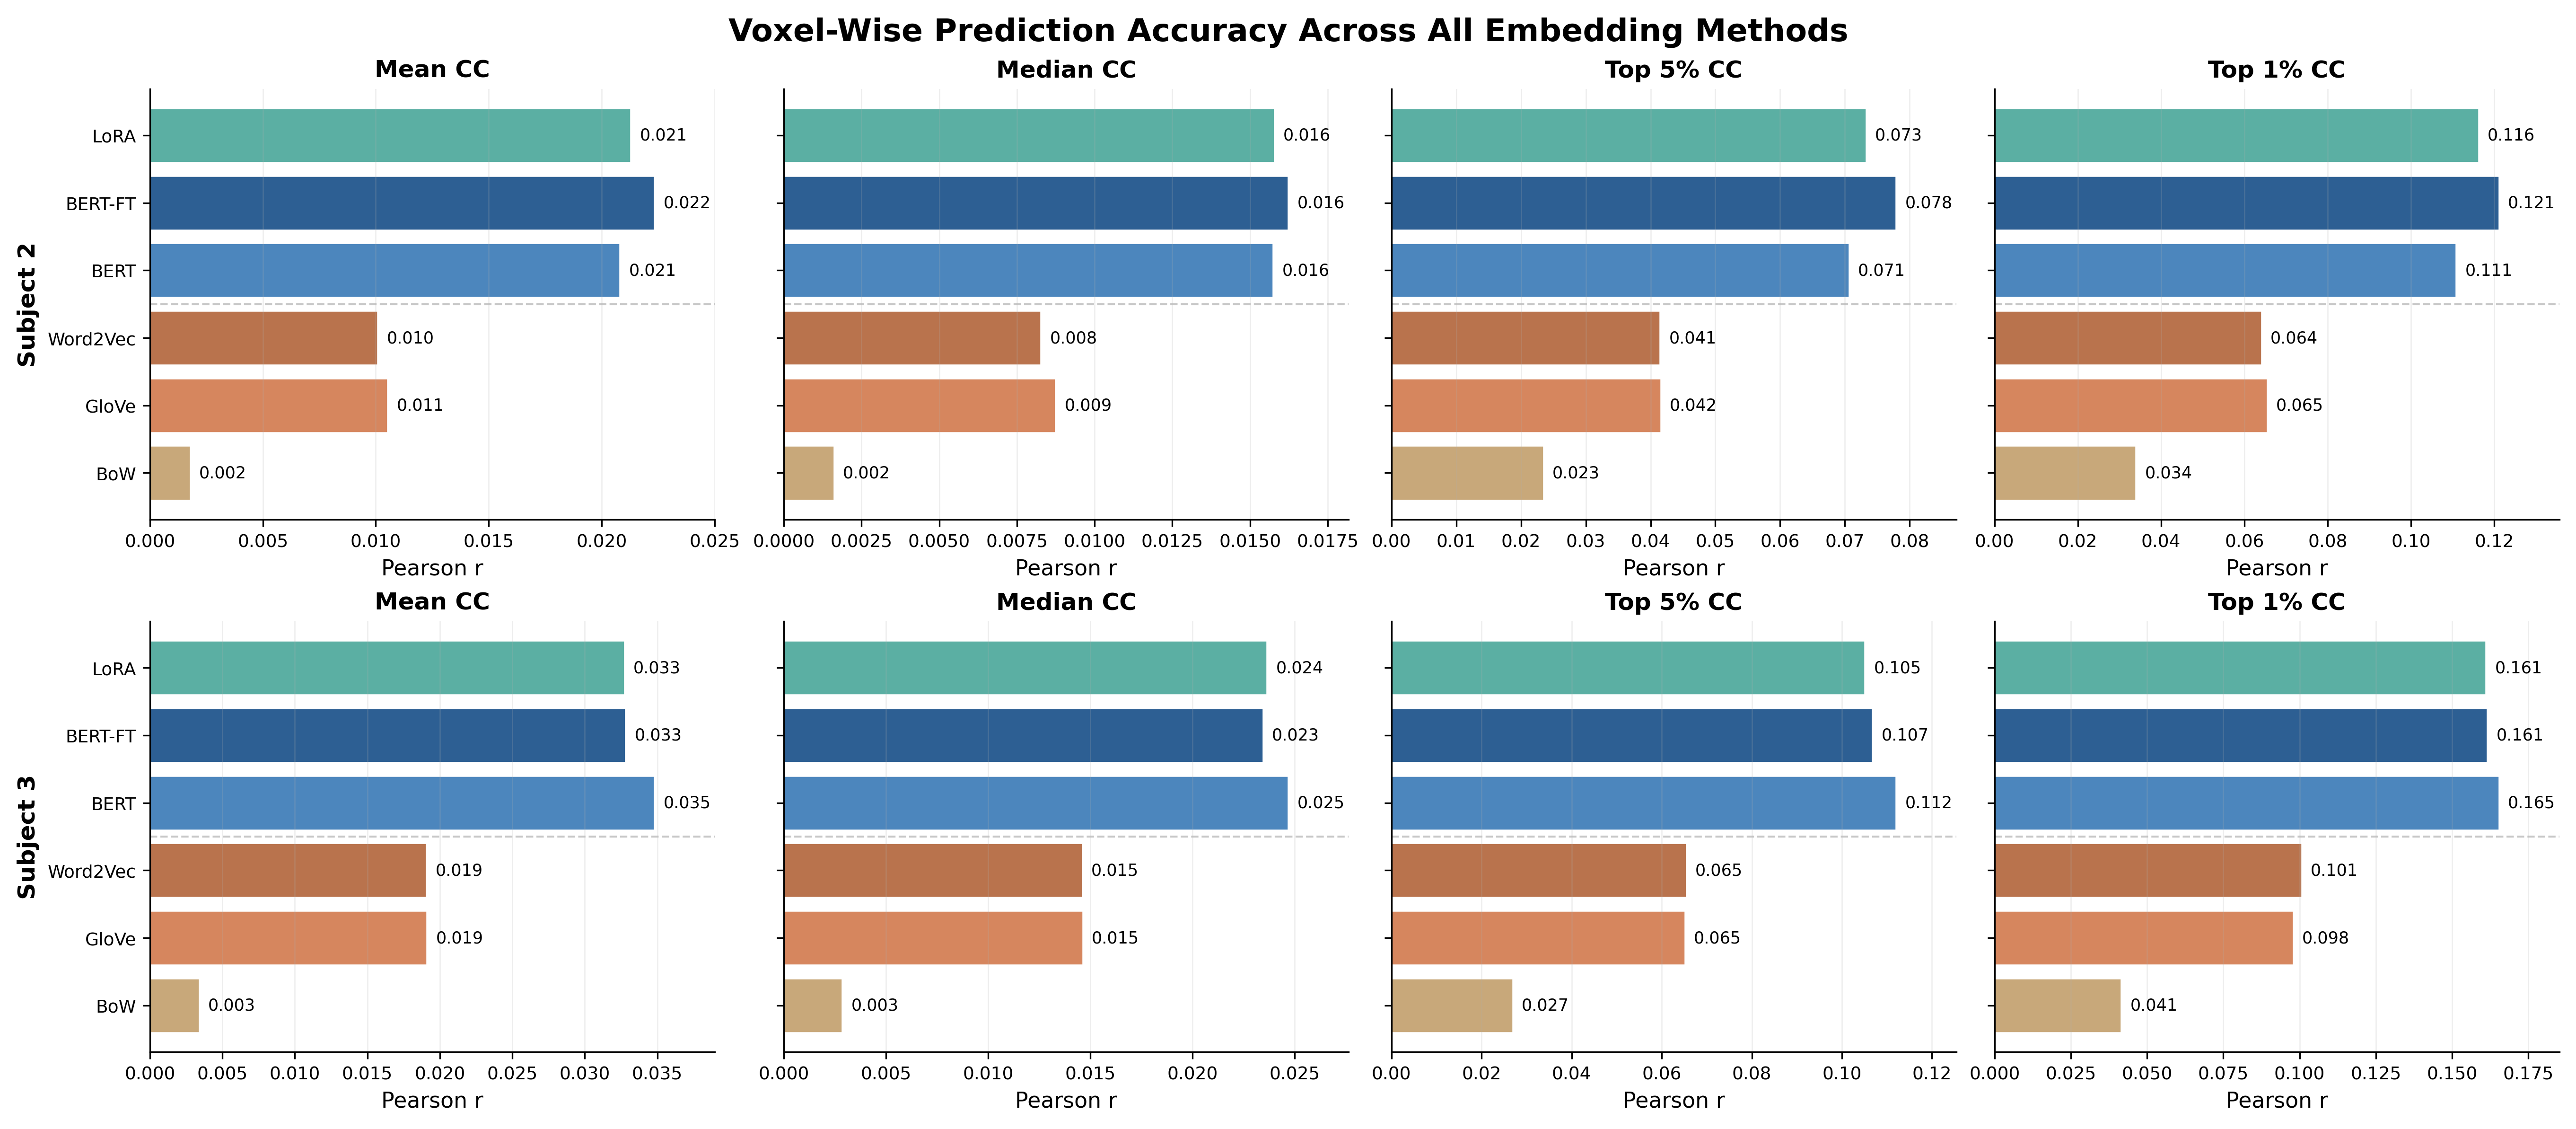
\includegraphics[width=\textwidth]{../figures/lab32/fig1_all_embeddings_hbars.png}
    \caption{Voxel-wise prediction accuracy across all six embedding methods, for Subject 2 (top) and Subject 3 (bottom). The ordering is consistent across all metrics and both subjects: BoW is weakest, GloVe and Word2Vec sit in the middle, and all three BERT variants are highest. Within the BERT family, pretrained BERT, BERT-FT, and LoRA have very similar CC values, so the choice among these fine-tuning strategies has a much smaller effect than the choice between static and contextual embeddings.}
    \label{fig:all_embeddings}
\end{figure}

Additionally, the jump to BERT is larger than the jump from BoW to static embeddings. Pretrained BERT achieves a mean CC of 0.0208 for Subject 2 and 0.0348 for Subject 3, with top 1\% CCs of 0.111 and 0.165, respectively. Compared with the best static embedding for each subject, this is roughly 60-70\% higher in the upper tail.

\subsection{How much does contextual representation help the best voxels?}

\begin{figure}[h]
    \centering
    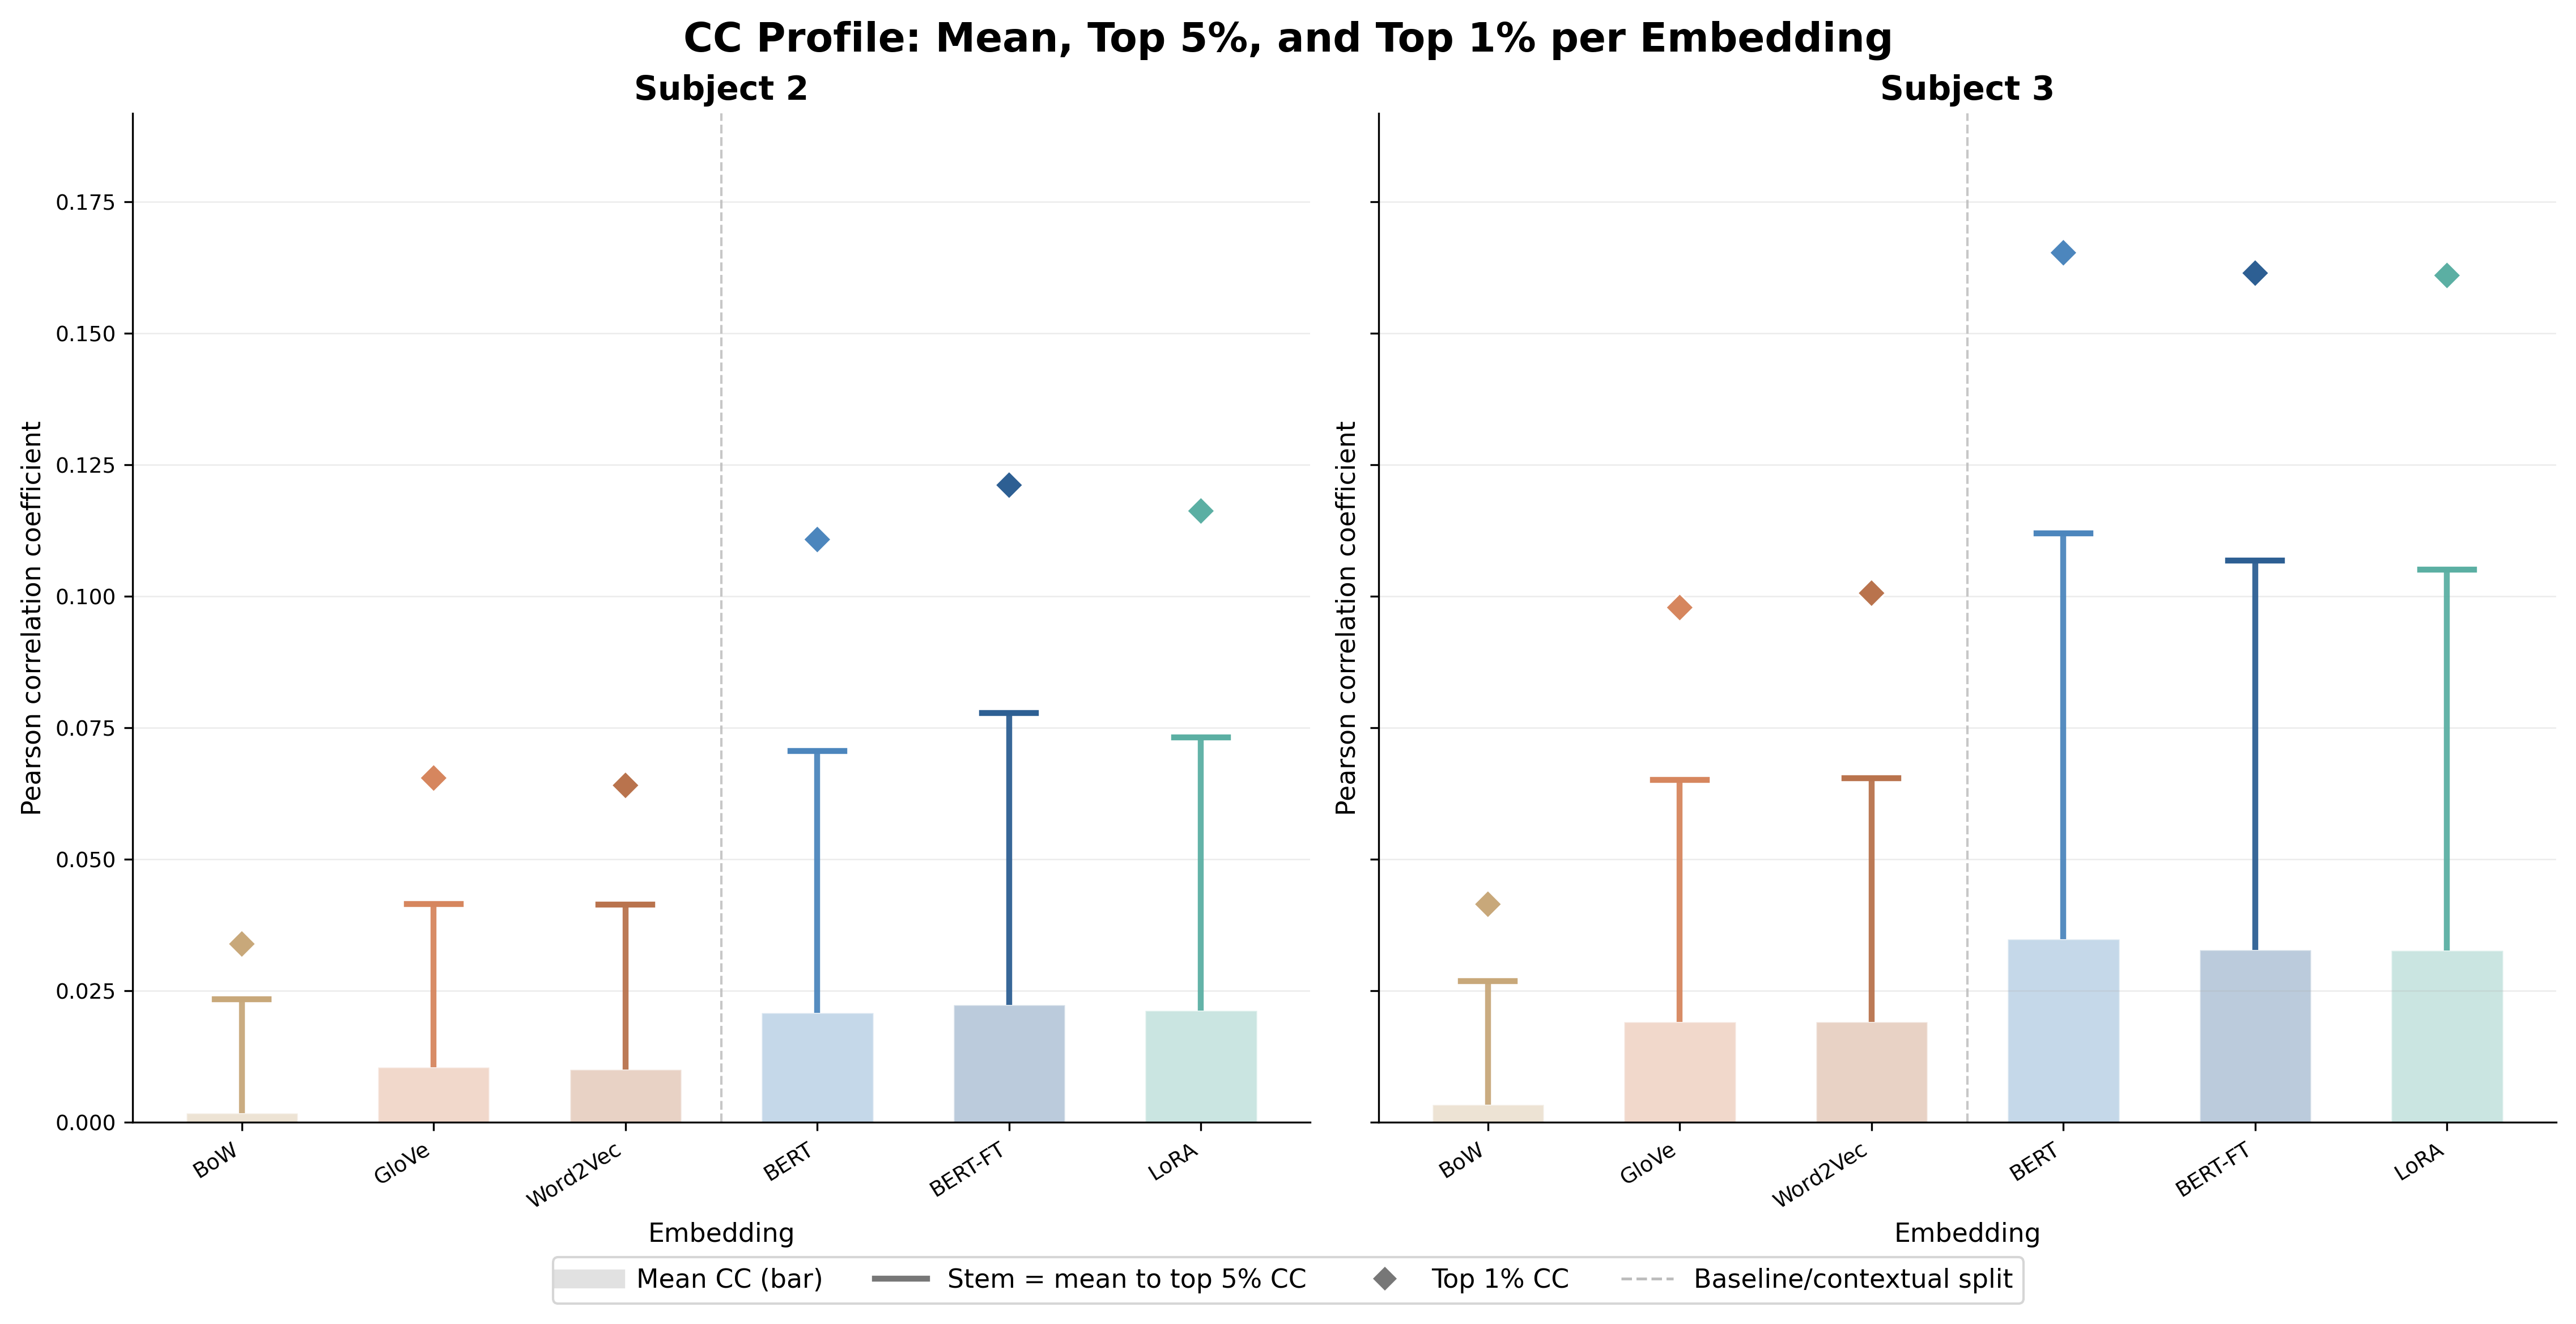
\includegraphics[width=\textwidth]{../figures/lab32/fig3_top_voxel_profiles.png}
    \caption{CC profiles for all six embedding methods, shown separately for Subject 2 (left) and Subject 3 (right). Each embedding is represented by a bar (mean CC), a vertical stem extending to the top 5\% CC, and a diamond marking the top 1\% CC. The dashed vertical line separates non-contextual from contextual methods. For Subject 2, BERT-FT achieves the highest top 1\% CC (0.121), followed by LoRA (0.116) and pretrained BERT (0.111). For Subject 3, pretrained BERT leads at 0.165, with BERT-FT and LoRA both around 0.161. The BERT-family models have a much heavier upper tail than the lexical and static embedding baselines.}
    \label{fig:cc_profile}
\end{figure}

The contextual advantage is strongest in the upper tail of the voxel-wise CC distribution. We can see this most clearly in Figure~\ref{fig:cc_profile}, which shows the mean CC, top 5\% CC, and top 1\% CC for each embedding method. The mean CC values are modest for every method, but the BERT-family models have much longer stems from mean CC to top 5\% CC and much higher top 1\% diamonds. This means that BERT's improvement is not spread evenly across all voxels. Instead, the largest gains occur among the voxels whose BOLD responses are already the most predictable from the language stimulus.

This pattern is important because most voxels are weakly predicted regardless of embedding method. If contextual embeddings were only adding small uniform gains across the brain, we would expect the upper-tail metrics to increase by roughly the same amount as the mean. Instead, the top 5\% and top 1\% metrics increase much more visibly. This suggests that contextual embeddings are especially useful for the subset of voxels that contain recoverable language-related signal. In other words, BERT does not make every voxel highly predictable, it makes the best-predicted voxels substantially better.

As an additional check, Appendix Figure~\ref{fig:contextual_lift_appendix} compares each BERT variant's top 1\% voxels with the best static embedding evaluated on those same voxels. The same pattern holds, contextual embeddings improve prediction even within the voxel subset where static embeddings already perform relatively well. This supports the interpretation that BERT is not only selecting a different favorable group of voxels, but is improving prediction for language-responsive voxels that are already somewhat predictable from static semantic features.

\subsection{Does fine-tuning help?}
From Table~\ref{tab:all-embedding-results}, the three BERT variants perform very similarly for both subjects. Specifically, fine-tuning gives a small improvement for Subject 2 in which BERT-FT has the highest top 1\% CC (0.1212) compared with pretrained BERT (0.1108). However, for Subject 3, pretrained BERT has the highest top 1\% CC (0.1653) compared with BERT-FT (0.1615). Since the best BERT variant changes by subject, and the differences among the three BERT models are much smaller than the gap between BERT and the non-BERT methods, fine-tuning does not appear to give a clear or reliable improvement.

Since the table averages over all voxels, it can hide what happens voxel-by-voxel. For example, one voxel could improve by $+0.05$ after fine-tuning while another worsens by $-0.05$, producing an average change near zero even though fine-tuning had a large effect on individual voxels. Figure~\ref{fig:delta} checks for this possibility by showing how much each voxel's held-out CC changes after fine-tuning, relative to pretrained BERT. If fine-tuning produced a strong systematic improvement, the histogram would shift clearly to the right of zero. If it produced large mixed effects, the histogram would be wide, with many voxels far from zero in both directions. Instead, all four distributions are narrow and centered close to zero. For Subject 2, BERT-FT improves 54.5\% of voxels with mean delta $+0.0015$, and LoRA improves 51.2\% with mean delta $+0.0005$. For Subject 3, the shifts go slightly in the opposite direction. BERT-FT improves 44.3\% of voxels with mean delta $-0.0020$, and LoRA improves 43.4\% with mean delta $-0.0021$.

\begin{figure}[H]
    \centering
    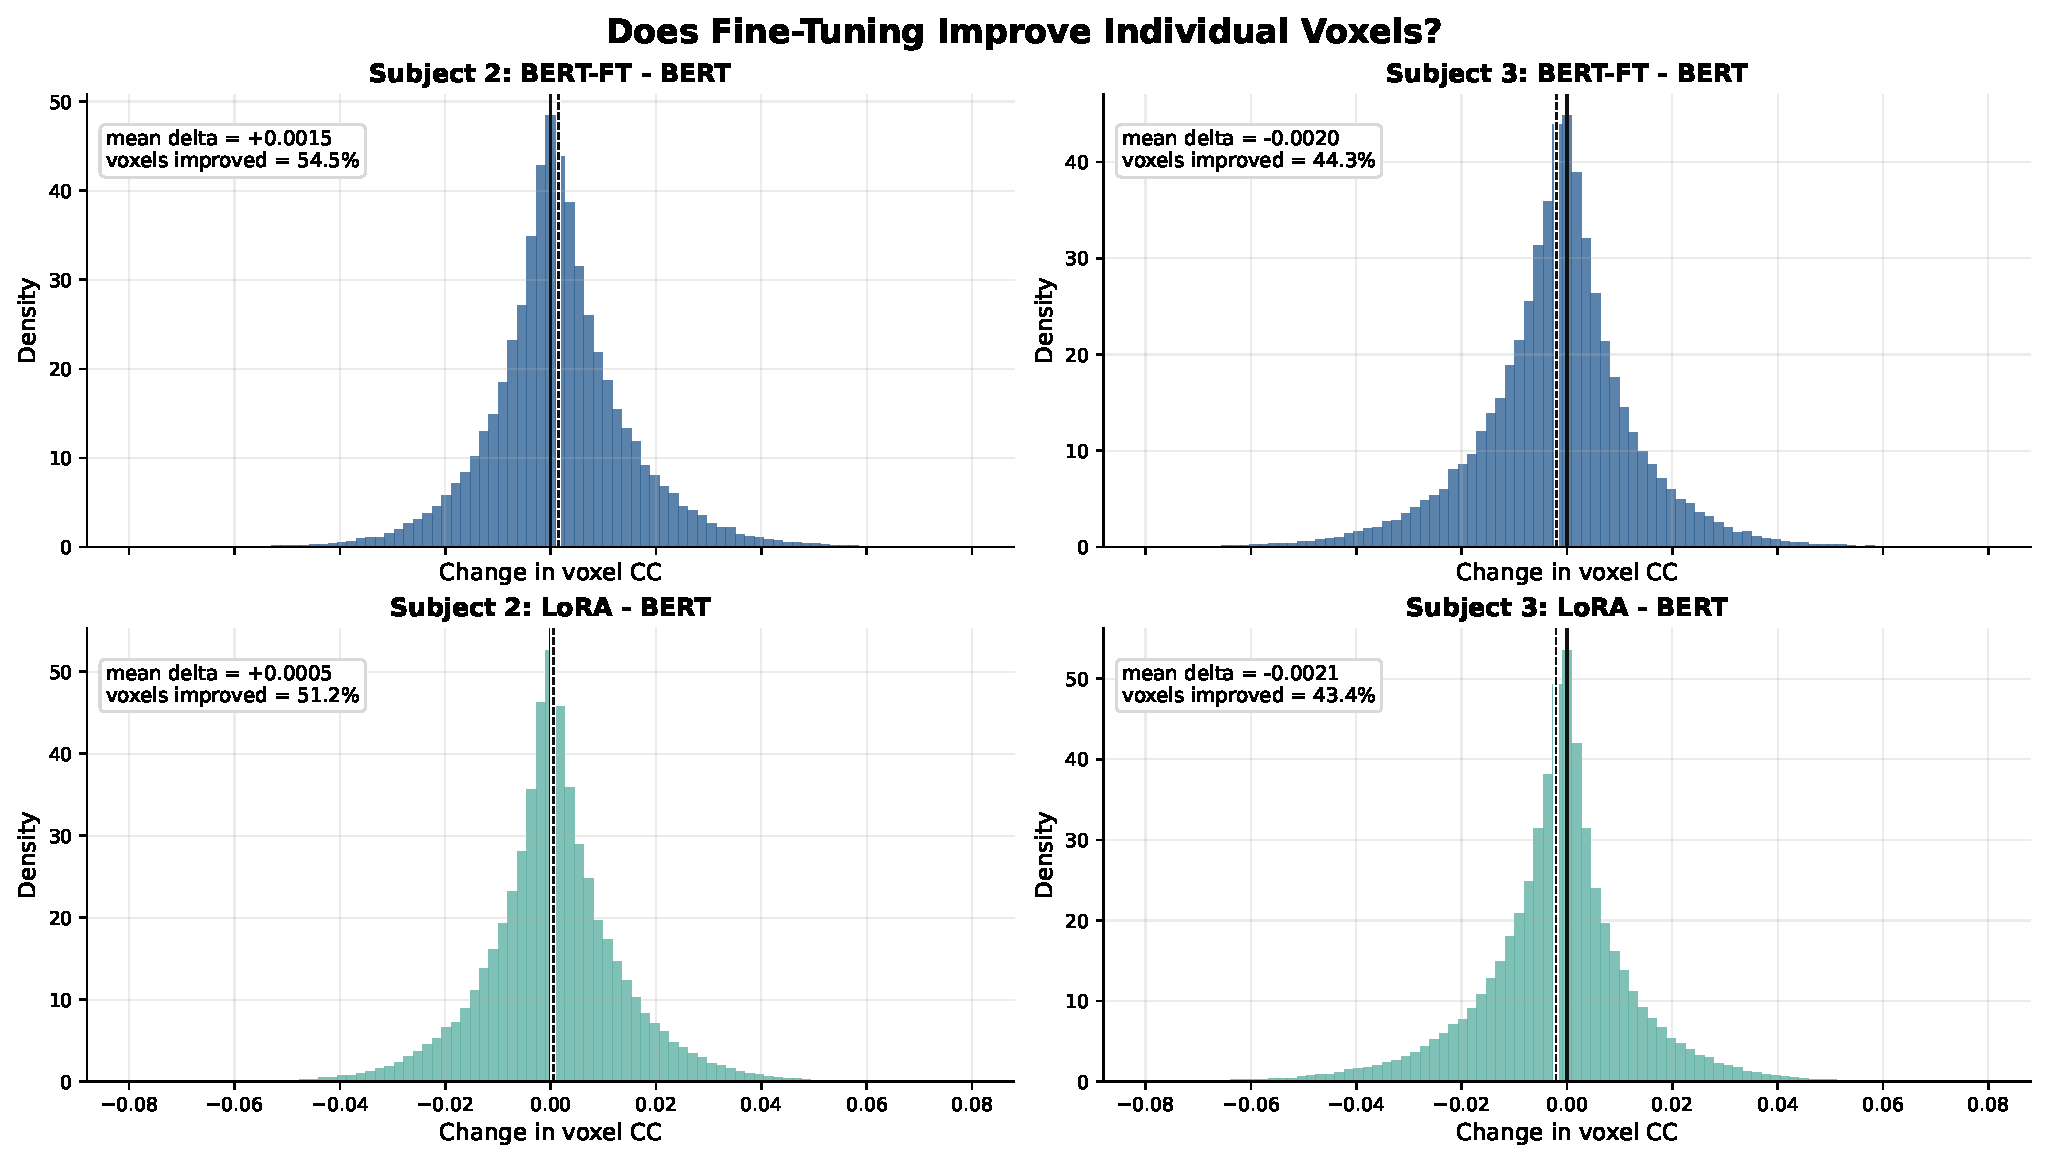
\includegraphics[width=\textwidth]{../figures/lab32/fig3_bert_delta_from_pretrained.pdf}
    \caption{Per-voxel change in held-out CC after fine-tuning, relative to pretrained BERT. Top row: BERT-FT minus BERT. Bottom row: LoRA minus BERT. Left column: Subject 2. Right column: Subject 3. The dashed line marks zero, and the solid line marks the mean delta. If fine-tuning produced a strong systematic improvement, the distributions would shift clearly to the right of zero. Instead, the distributions are narrow and centered near zero. Subject 2 shows a small positive shift, while Subject 3 shows a small negative shift. This indicates that fine-tuning has only a weak and subject-dependent effect on voxel-wise prediction.}
    \label{fig:delta}
\end{figure}

Thus, fine-tuning changes many voxel predictions slightly, but it does not produce a large or consistent improvement over pretrained BERT. Although pretrained BERT remained highly competitive, we used fine-tuned BERT for SHAP and LIME so that the interpretation focused on the task-adapted model.

\subsection{Are the two subjects consistent?}
Although the ordering of embedding methods is similar across subjects, Subject 3 is generally more predictable than Subject 2. Previously, Table~\ref{tab:all-embedding-results} shows that Subject 3 has higher CC values than Subject 2 for every embedding method and summary metric. The difference between Subject 3 and Subject 2 is small for BoW, but it becomes larger for contextual embeddings. Under pretrained BERT, mean CC increases from 0.0208 for Subject 2 to 0.0348 for Subject 3, and top 1\% CC increases from 0.111 to 0.165. This pattern can be seen in Figure~\ref{fig:subject_consistency}. Each point represents one embedding method, with Subject 2 performance on the x-axis and Subject 3 performance on the y-axis. Points above the diagonal indicate higher performance for Subject 3. The figure again supports the earlier result that contextual embeddings outperform static embeddings for both subjects: BoW is lowest, GloVe and Word2Vec are intermediate, and the BERT variants are highest. GloVe and Word2Vec are nearly overlapping in every panel, suggesting that the two static semantic embeddings behave very similarly in this encoding pipeline.

\begin{figure}[H]
    \centering
    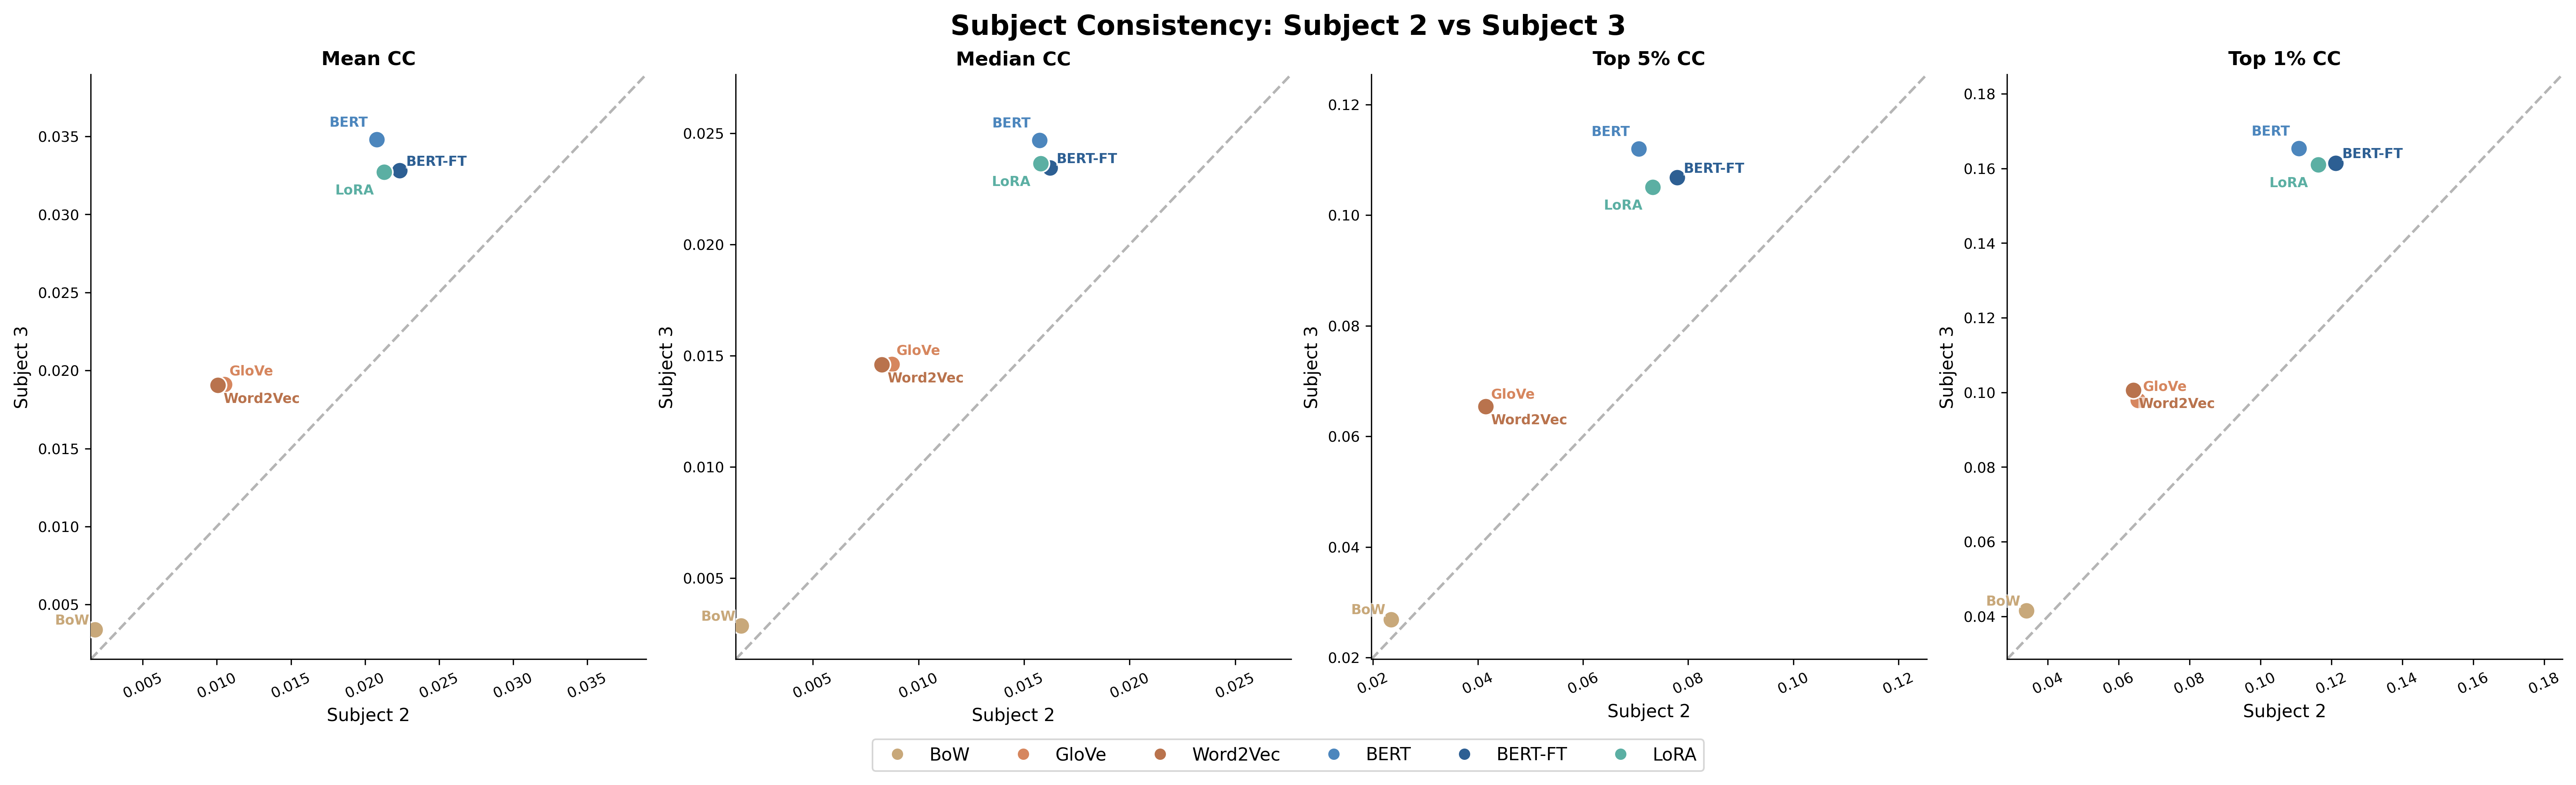
\includegraphics[width=\textwidth]{../figures/lab32/fig4_subject_consistency.png}
    \caption{Method-level cross-subject consistency across all four CC metrics. Each point is one embedding method, with Subject 2 on the x-axis and Subject 3 on the y-axis. Points above the dashed diagonal indicate higher performance for Subject 3. The BERT-family points sit farther above the diagonal, showing that Subject 3's advantage is largest for the best-performing contextual models. The three BERT variants cluster tightly together in all panels, suggesting that fine-tuning choice has a smaller effect than the broader distinction between static and contextual embeddings.}
    \label{fig:subject_consistency}
\end{figure}

The figure also shows that the size of the BERT improvement is not exactly the same for the two subjects. Since Subject 2 is on the x-axis and Subject 3 is on the y-axis, movement to the right reflects improvement for Subject 2, while movement upward reflects improvement for Subject 3. The BERT cluster is farther above the static-embedding cluster than it is to the right of it, so the gain from contextual embeddings appears larger for Subject 3. This does not change the main conclusion that BERT performs best for both subjects, but it shows that the amount of improvement can vary by subject.

\subsection{Which words matter most, and do SHAP and LIME agree?}
\label{sec:interpretability-results}
\paragraph{Selecting Voxels for Interpretation} Because most voxels are weakly predicted, we restricted SHAP and LIME to high-CC voxels. Appendix Figure~\ref{fig:bert_distributions_appendix} shows the full voxel-wise CC distributions for the BERT variants and confirms that reliable prediction is concentrated in the upper tail rather than spread across the whole brain. We used fine-tuned BERT for the SHAP and LIME analyses because it was one of the strongest BERT-family models and allowed us to interpret the model after task-specific language adaptation. The two held-out test stories we selected were \textit{Can Planet Earth Feed Ten Billion People? Part 1} and \textit{Stumbling in the Dark}, and we interpreted the top 3 voxels for each subject. The selected voxels all had held-out story CC values above 0.10. For each selected story and voxel, we used the wrapper-style SHAP and LIME procedure described in Section~\ref{sec:interpretation-methods} to perturb words in the original story and measure how those perturbations changed the voxel's story-level prediction quality. Figure~\ref{fig:dual_importance_both_stories} shows the top-ranked SHAP words and the corresponding LIME importances for the three highest-CC voxels per subject in each story.

The selected voxels have story-level CC values around 0.28-0.39, which are high relative to the overall voxel-wise prediction distribution. These values make the voxels reasonable targets for

\begin{figure}[H]
    \centering

    \begin{subfigure}{\textwidth}
        \centering
        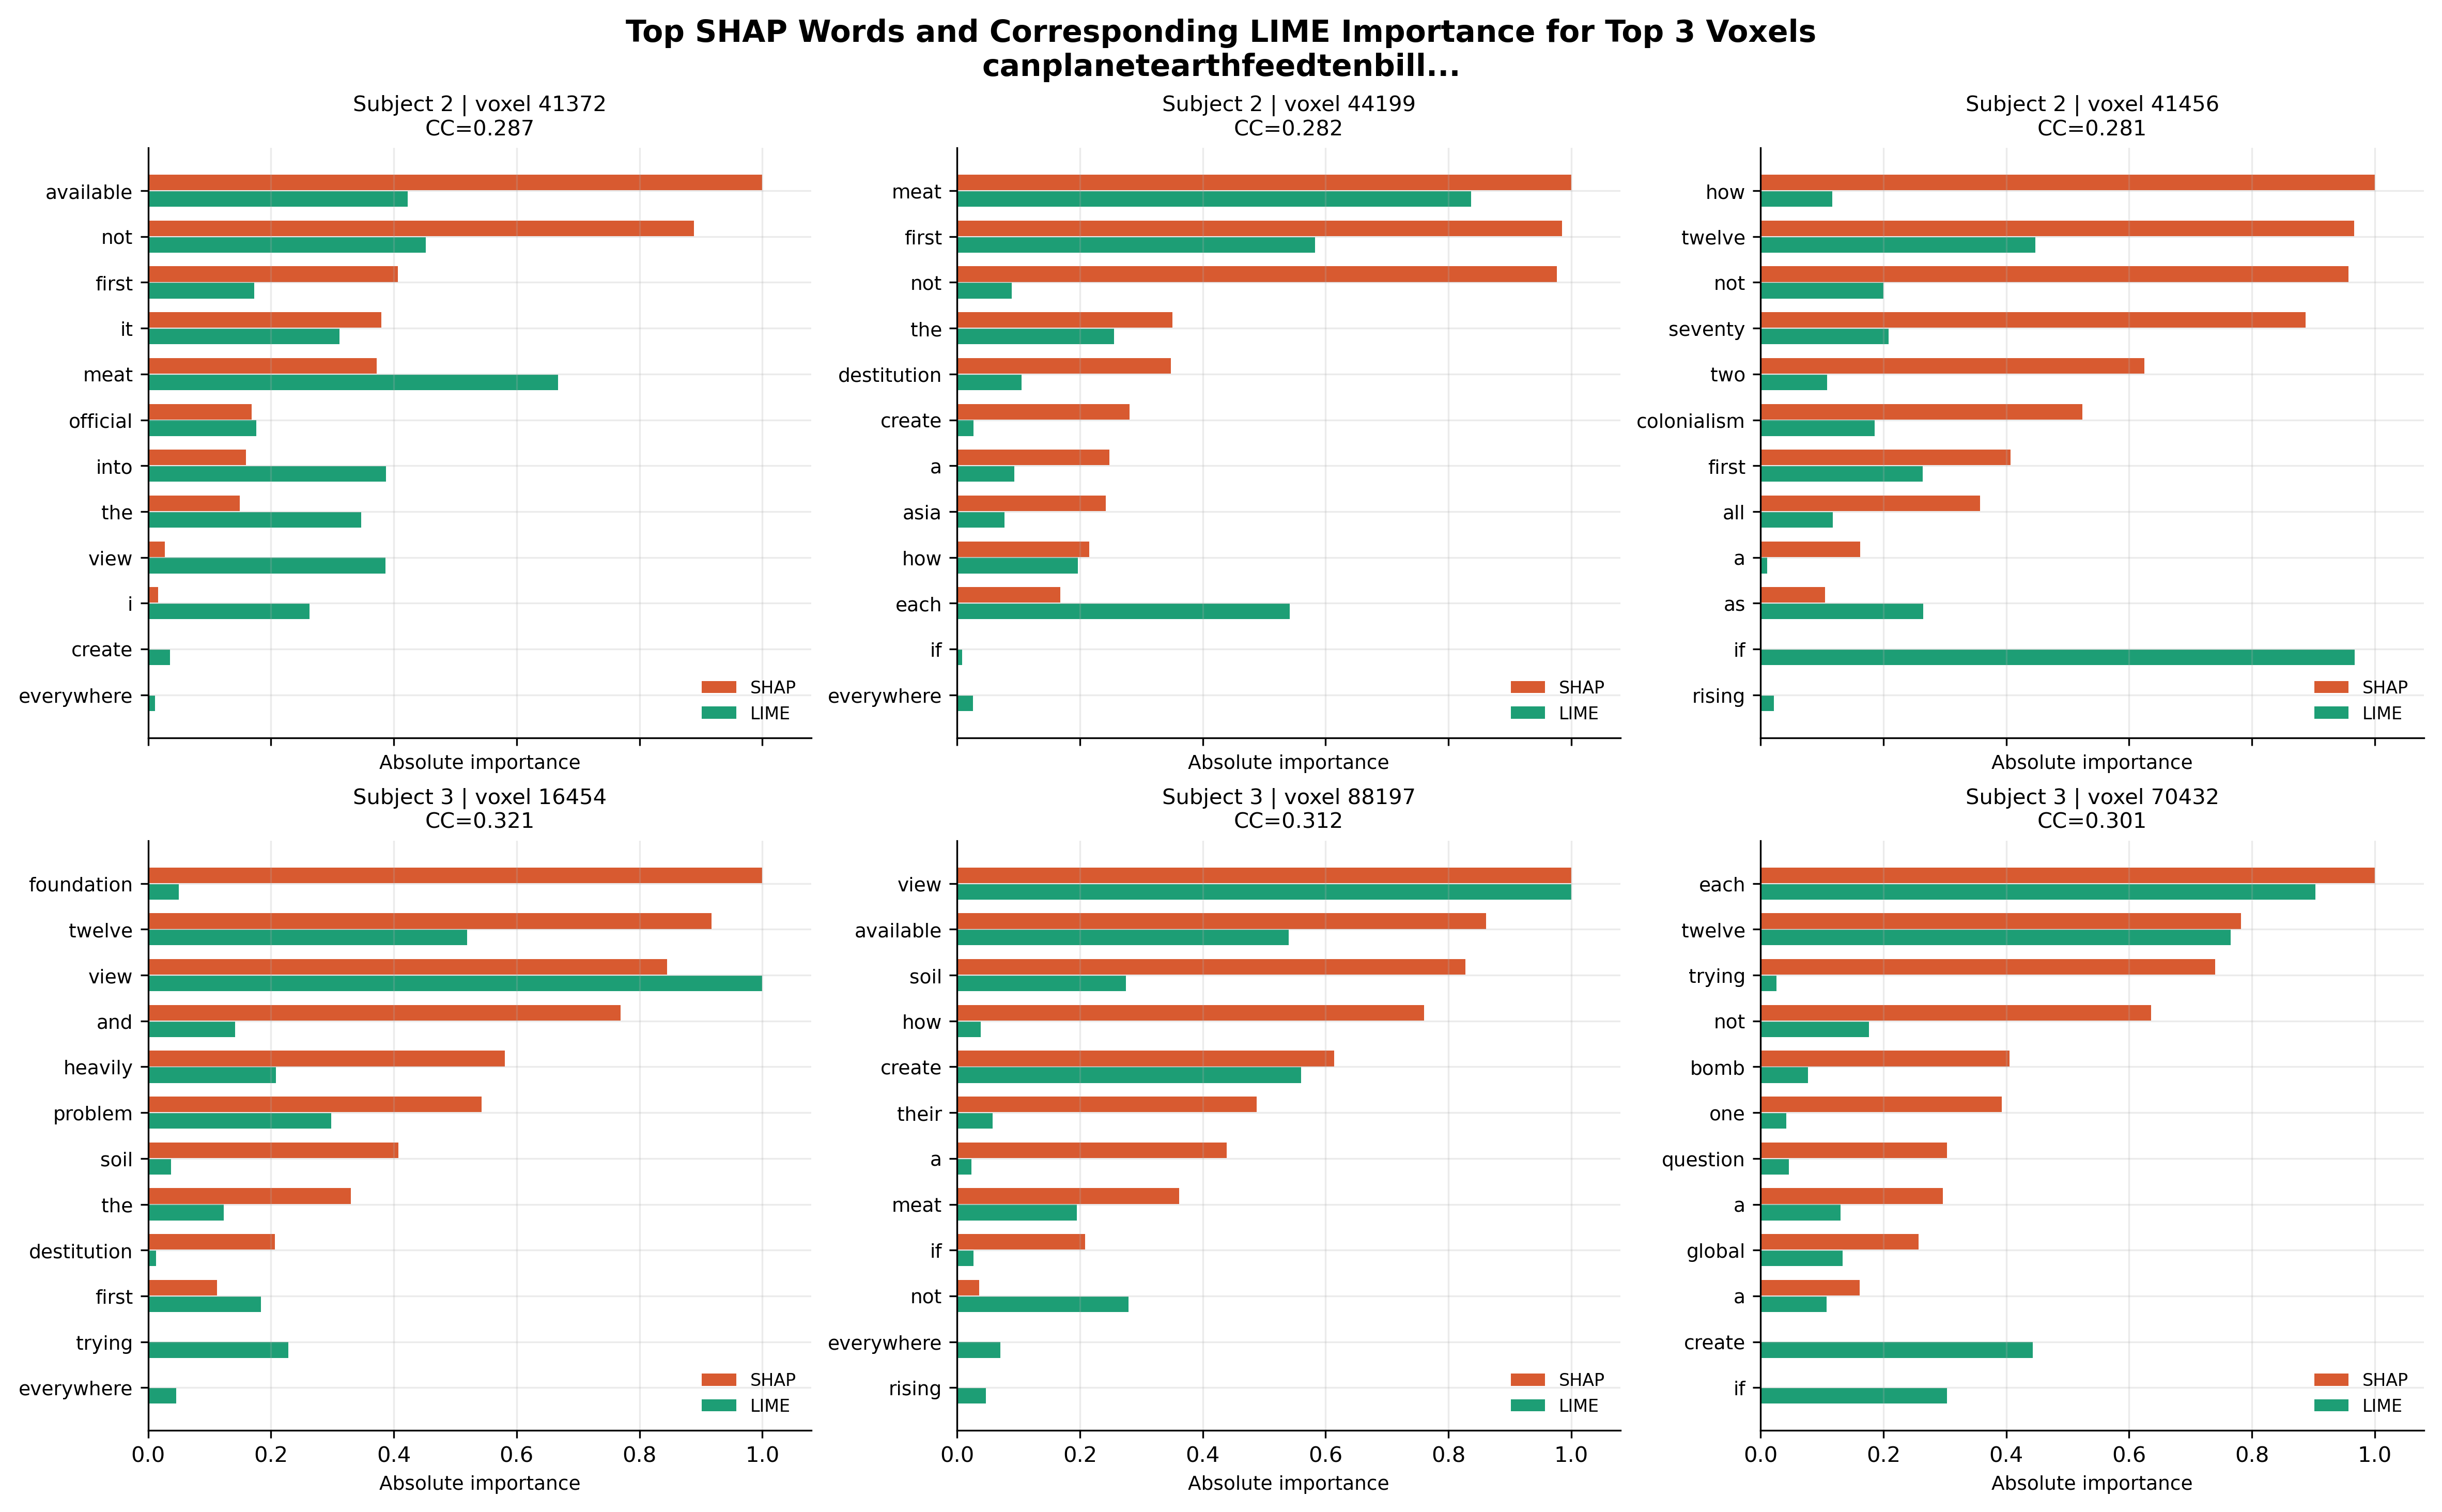
\includegraphics[width=\textwidth]{../figures/lab33/fig1_dual_importance_story1.png}
        \label{fig:importance_story1}
    \end{subfigure}
    
    \begin{subfigure}{\textwidth}
        \centering
        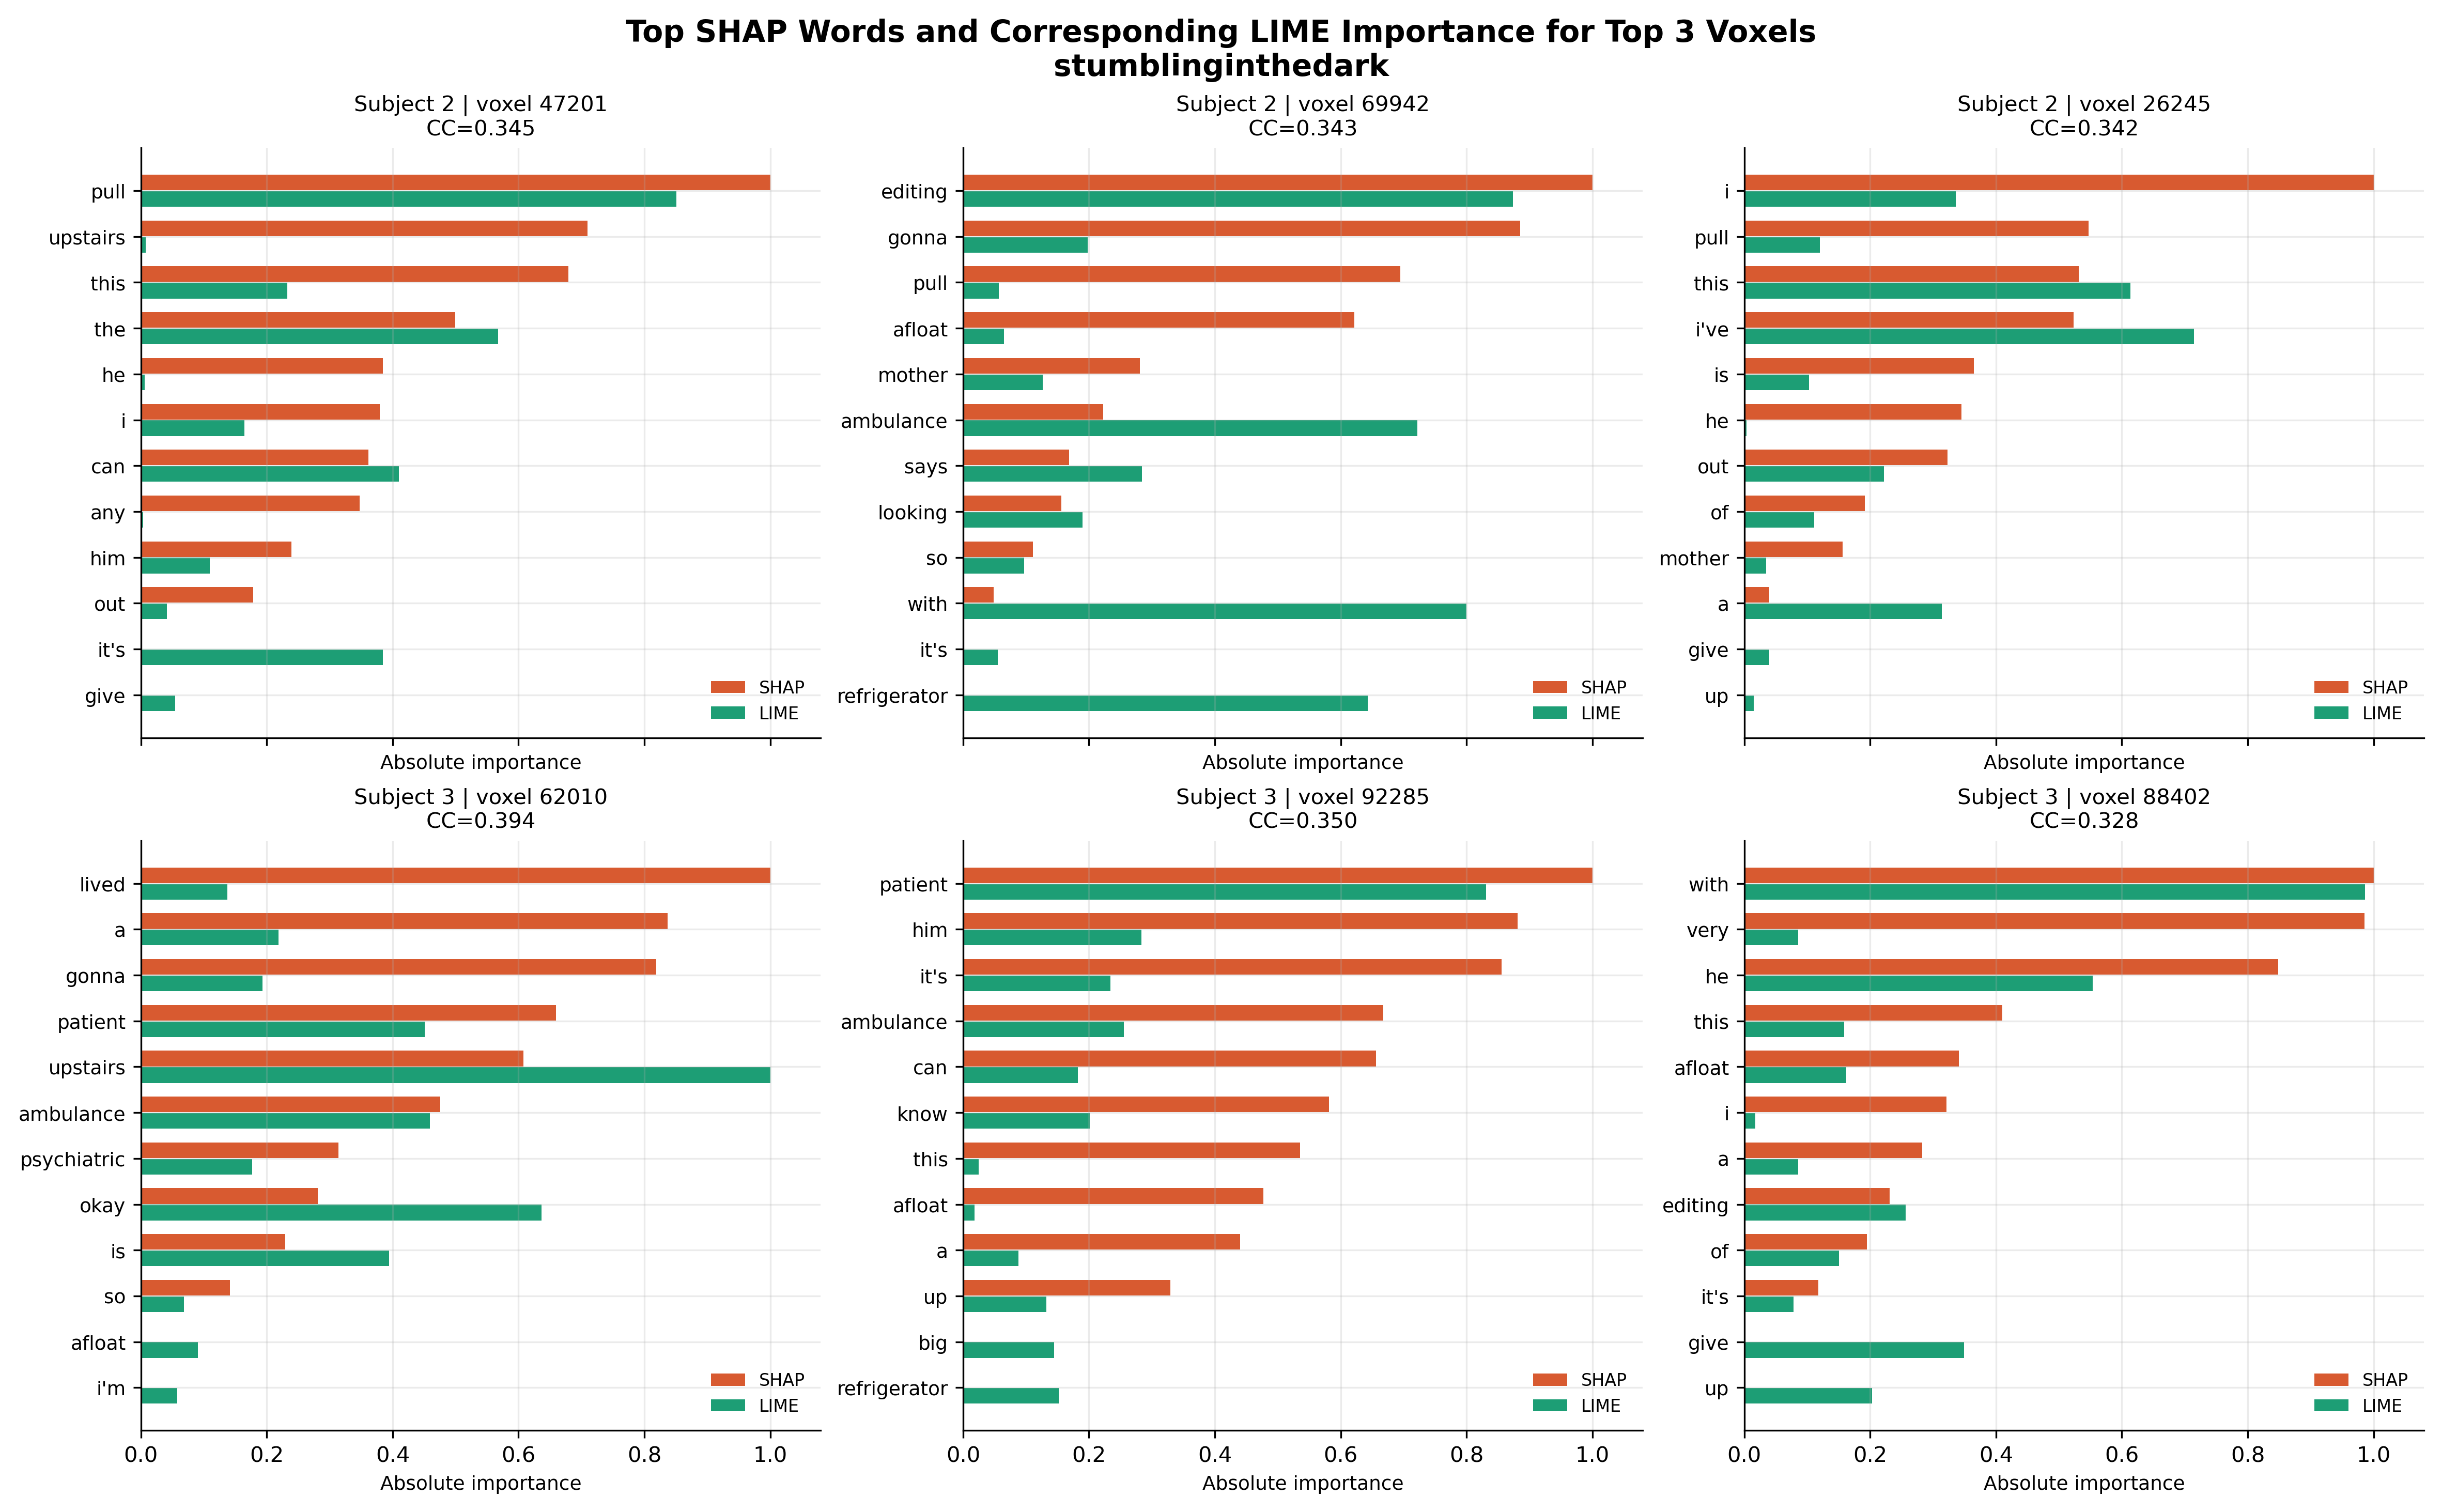
\includegraphics[width=\textwidth]{../figures/lab33/fig1_dual_importance_story2.png}
        \label{fig:importance_story2}
    \end{subfigure}

    \caption{Top SHAP words and corresponding LIME importances for the three highest-CC voxels per subject in each interpreted story. Words are ranked by absolute SHAP importance and normalized within each voxel. Both stories show a mix of interpretable content words and generic/function words. SHAP/LIME agreement is partial and varies across voxels.}
    \label{fig:dual_importance_both_stories}
\end{figure}

interpretation, although they should still be understood as modest correlations in the broader context of noisy fMRI prediction. Across both stories, some high-ranked words are more interpretable than others. SHAP and LIME often identify function words or short common words such as \textit{not}, \textit{it}, \textit{the}, \textit{a}, \textit{if}, \textit{i}, \textit{he}, \textit{is}, \textit{can}, \textit{this}, and \textit{with}. We therefore do not interpret every high-ranked token as a semantic concept. These words may matter because they affect sentence structure, BERT context, or nearby narrative content, rather than because the word itself has a clear standalone meaning.

At the same time, several top words are semantically tied to the stories. In \textit{canplanetearthfeedtenbillionpeople}, words such as \textit{available}, \textit{meat}, \textit{destitution}, \textit{colonialism}, \textit{soil}, \textit{global}, \textit{problem}, \textit{foundation}, and \textit{bomb} connect to the story's themes of food systems, scarcity, inequality, agriculture, and global development. In \textit{stumblinginthedark}, words such as \textit{pull}, \textit{upstairs}, \textit{editing}, \textit{ambulance}, \textit{patient}, \textit{refrigerator}, \textit{lived}, \textit{mother}, \textit{afloat}, and \textit{psychiatric} are more connected to the story's personal and event-based narrative. These patterns suggest that the explanations capture some story-relevant content, although there is still a noticeable presence of function words.

Overall, SHAP and LIME show limited agreement. The bar plots reveal some shared high-importance words within individual voxels, but they also show many cases where one method assigns a word high importance while the other method assigns it little or no importance. For \textit{canplanetearthfeedtenbillionpeople}, the top voxels identify some thematically meaningful words, but the exact words vary across voxels and subjects. For \textit{stumblinginthedark}, there are several plausible event-related words, and some Subject 3 voxels show local SHAP/LIME agreement, but the agreement is not strong enough to treat the two methods as interchangeable.

\begin{figure}[H]
    \centering
    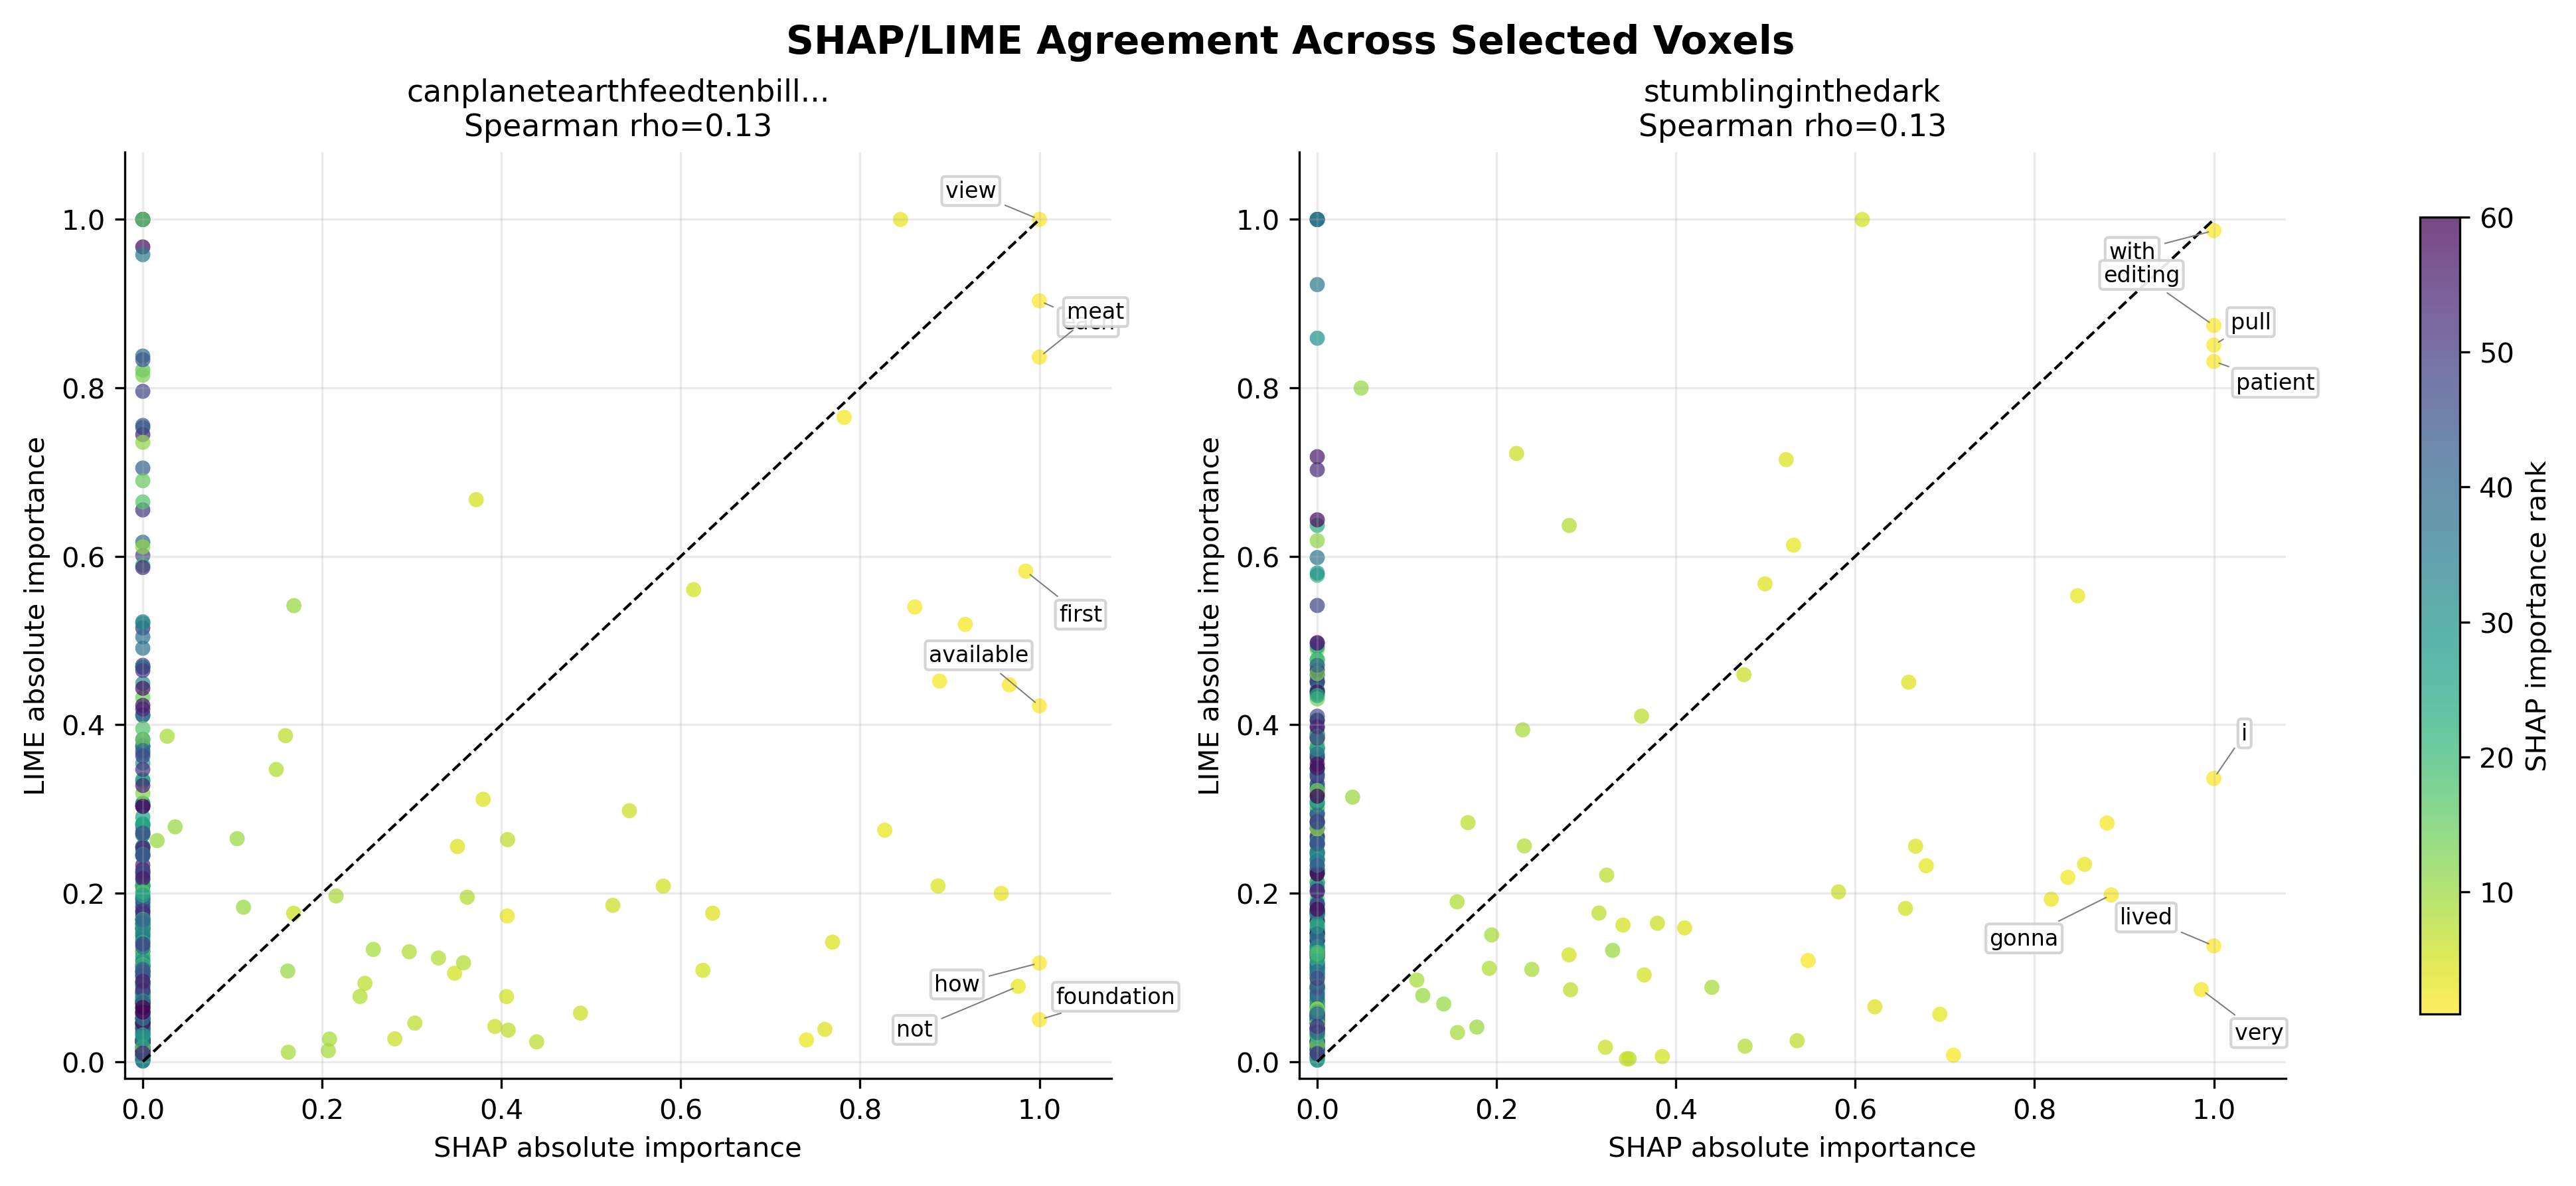
\includegraphics[width=\textwidth]{../figures/lab33/fig2_shap_lime_agreement_by_story.png}
    \caption{SHAP versus LIME word-importance agreement for the two interpreted stories. Each point represents one candidate word for one selected voxel. The x-axis shows normalized absolute SHAP importance, and the y-axis shows normalized absolute LIME importance. The dashed line marks equal importance under both methods. Only a subset of high-importance words is labeled to avoid text overlap, but all candidate words are included in the scatter and in the Spearman correlation. Agreement is low for both stories, with Spearman \(\rho=0.13\) for \textit{canplanetearthfeedtenbillionpeople} and \(\rho=0.13\) for \textit{stumblinginthedark}. The large number of points far from the diagonal shows that SHAP and LIME often assign importance differently.}
    \label{fig:agreement}
\end{figure}

This pattern is also visible in Figure~\ref{fig:agreement}, which compares SHAP and LIME importances across candidate words. The overall rank agreement is low for both stories, with Spearman \(\rho=0.13\) for \textit{canplanetearthfeedtenbillionpeople} and \(\rho=0.13\) for \textit{stumblinginthedark}. In both panels, many points lie far from the diagonal. Some words have high SHAP importance but low LIME importance, such as \textit{how}, \textit{foundation}, and \textit{not} in the food story, or \textit{gonna}, \textit{lived}, and \textit{very} in the personal story. Conversely, some words receive high LIME importance despite low SHAP importance. This suggests that the two methods capture different aspects of the perturbation behavior, and words identified by both methods should be treated as more stable than words identified by only one.

As an additional check on whether word effects were shared across selected voxels, we also examined heatmaps of signed SHAP values (Appendix Figures~\ref{fig:heatmap_story1_appendix} and~\ref{fig:heatmap_story2_appendix}). These heatmaps further support the voxel-specific interpretation above. For example, in \textit{stumblinginthedark}, \textit{upstairs}, \textit{patient}, and \textit{editing} are story-relevant words and appear among the top words in the bar plots, but their signed SHAP effects are not consistent across all selected voxels. Similarly, in \textit{canplanetearthfeedtenbillionpeople}, \textit{meat}, \textit{soil}, and \textit{foundation} are semantically meaningful and important for some voxels, but they do not show consistent signed effects across both subjects. Thus, the heatmaps reinforce our main caution mentioned earlier, and that is the explanations identify plausible story-relevant words, but the exact word effects are voxel-specific rather than general brain-wide language effects.

\section{Stability Analyses}
Following the PCS framework \cite{yu2024}, we performed stability analyses for two modeling choices that could affect our conclusions. First, we tested whether BERT's advantage depends on using surrounding story context when extracting embeddings. Second, we tested whether the LoRA results are sensitive to the adapter rank. Together, these checks help us evaluate whether our main findings are stable across reasonable alternatives.

\subsection{Does BERT Need Story Context?}
\label{sec:stability-context}
One important modeling choice was how to extract BERT embeddings from each story. Our main BERT pipeline gives BERT surrounding story context when representing each word, so the resulting embeddings reflect how the word is used in the narrative. As a stability check, we compared this choice against a word-level BERT baseline, where BERT-derived embeddings are extracted with much less surrounding context. This comparison asks whether the surrounding story context used during embedding extraction improves prediction, or whether BERT-derived word vectors with limited context are enough.

\begin{table}[H]
\centering
\begin{tabular}{llrrrr}
\toprule
Subject & Model & Mean CC & Median CC & Top 5\% CC & Top 1\% CC \\
\midrule
Subject 2 & Word-level BERT & 0.0089 & 0.0078 & 0.0364 & 0.0587 \\
Subject 2 & Contextual BERT & 0.0208 & 0.0157 & 0.0706 & 0.1108 \\
Subject 2 & Gain & +0.0119 & +0.0080 & +0.0342 & +0.0521 \\
\midrule
Subject 3 & Word-level BERT & 0.0185 & 0.0148 & 0.0611 & 0.0963 \\
Subject 3 & Contextual BERT & 0.0348 & 0.0247 & 0.1120 & 0.1653 \\
Subject 3 & Gain & +0.0163 & +0.0098 & +0.0509 & +0.0691 \\
\bottomrule
\end{tabular}
\caption{Stability check comparing word-level BERT with contextual BERT. Values are voxel-wise held-out CC summaries. Contextual BERT uses surrounding story context during embedding extraction, while word-level BERT uses much less context.}
\label{tab:wordlevel-contextual-stability}
\end{table}

Table~\ref{tab:wordlevel-contextual-stability} shows that contextual BERT outperforms the word-level BERT baseline for both subjects and across all four CC metrics. For Subject 2, mean CC increases from 0.0089 to 0.0208, and top 1\% CC increases from 0.0587 to 0.1108. For Subject 3, mean CC increases from 0.0185 to 0.0348, and top 1\% CC increases from 0.0963 to 0.1653. Therefore, the improvement is not limited to one subject or one summary metric.

\begin{figure}[h]
    \centering
    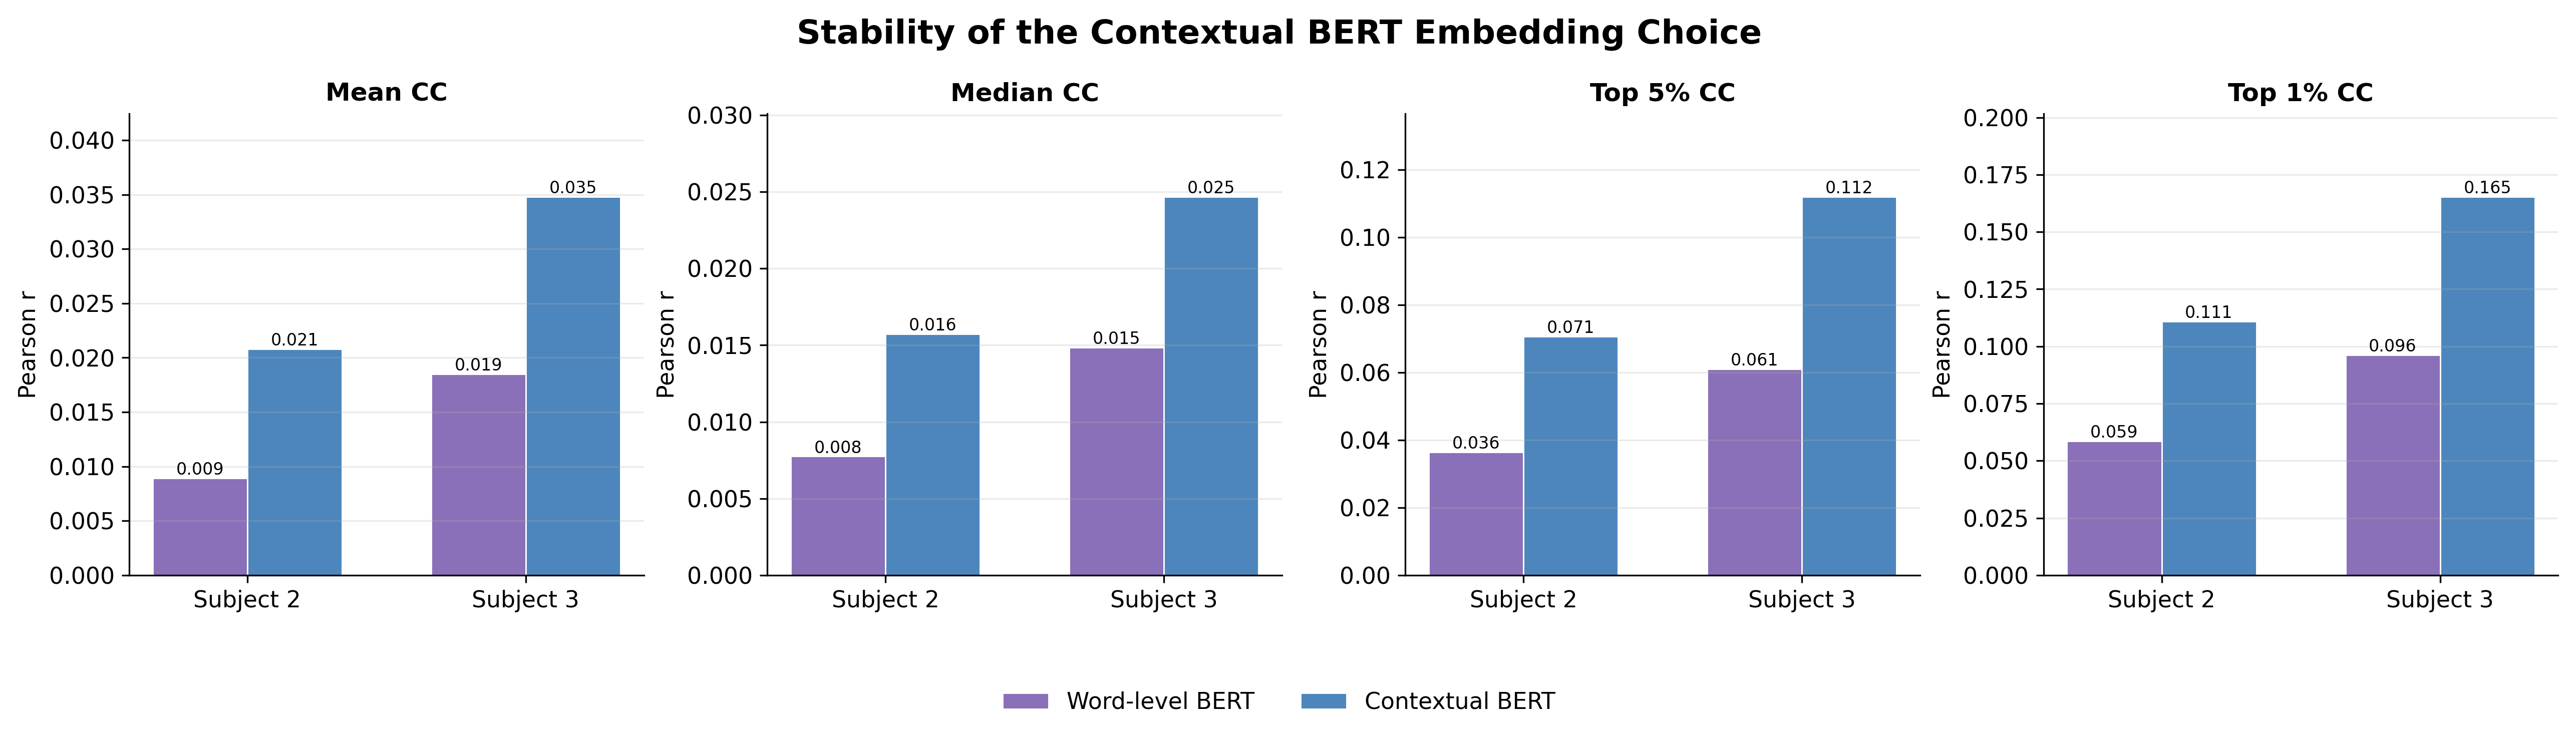
\includegraphics[width=\textwidth]{../figures/lab32/stability_contextual_vs_wordlevel_metrics.png}
    \caption{Stability check comparing word-level BERT and contextual BERT across CC summary metrics. Contextual BERT performs better for both subjects across mean CC, median CC, top 5\% CC, and top 1\% CC. The improvement is especially clear in the top-percentile metrics, indicating that surrounding story context increases performance most in the high-CC tail of the voxel distribution.}
    \label{fig:context-stability-metrics}
\end{figure}

Similarly, Figure~\ref{fig:context-stability-metrics} shows that the contextual BERT bars are higher than the word-level BERT bars in every panel. The gap is largest in the top-percentile metrics, especially top 5\% and top 1\% CC. This matters scientifically because these high-CC voxels are the voxels we later consider most appropriate for interpretation. In other words, contextual information helps most in the subset of voxels where the language encoding model is most reliable.

\begin{figure}[H]
    \centering
    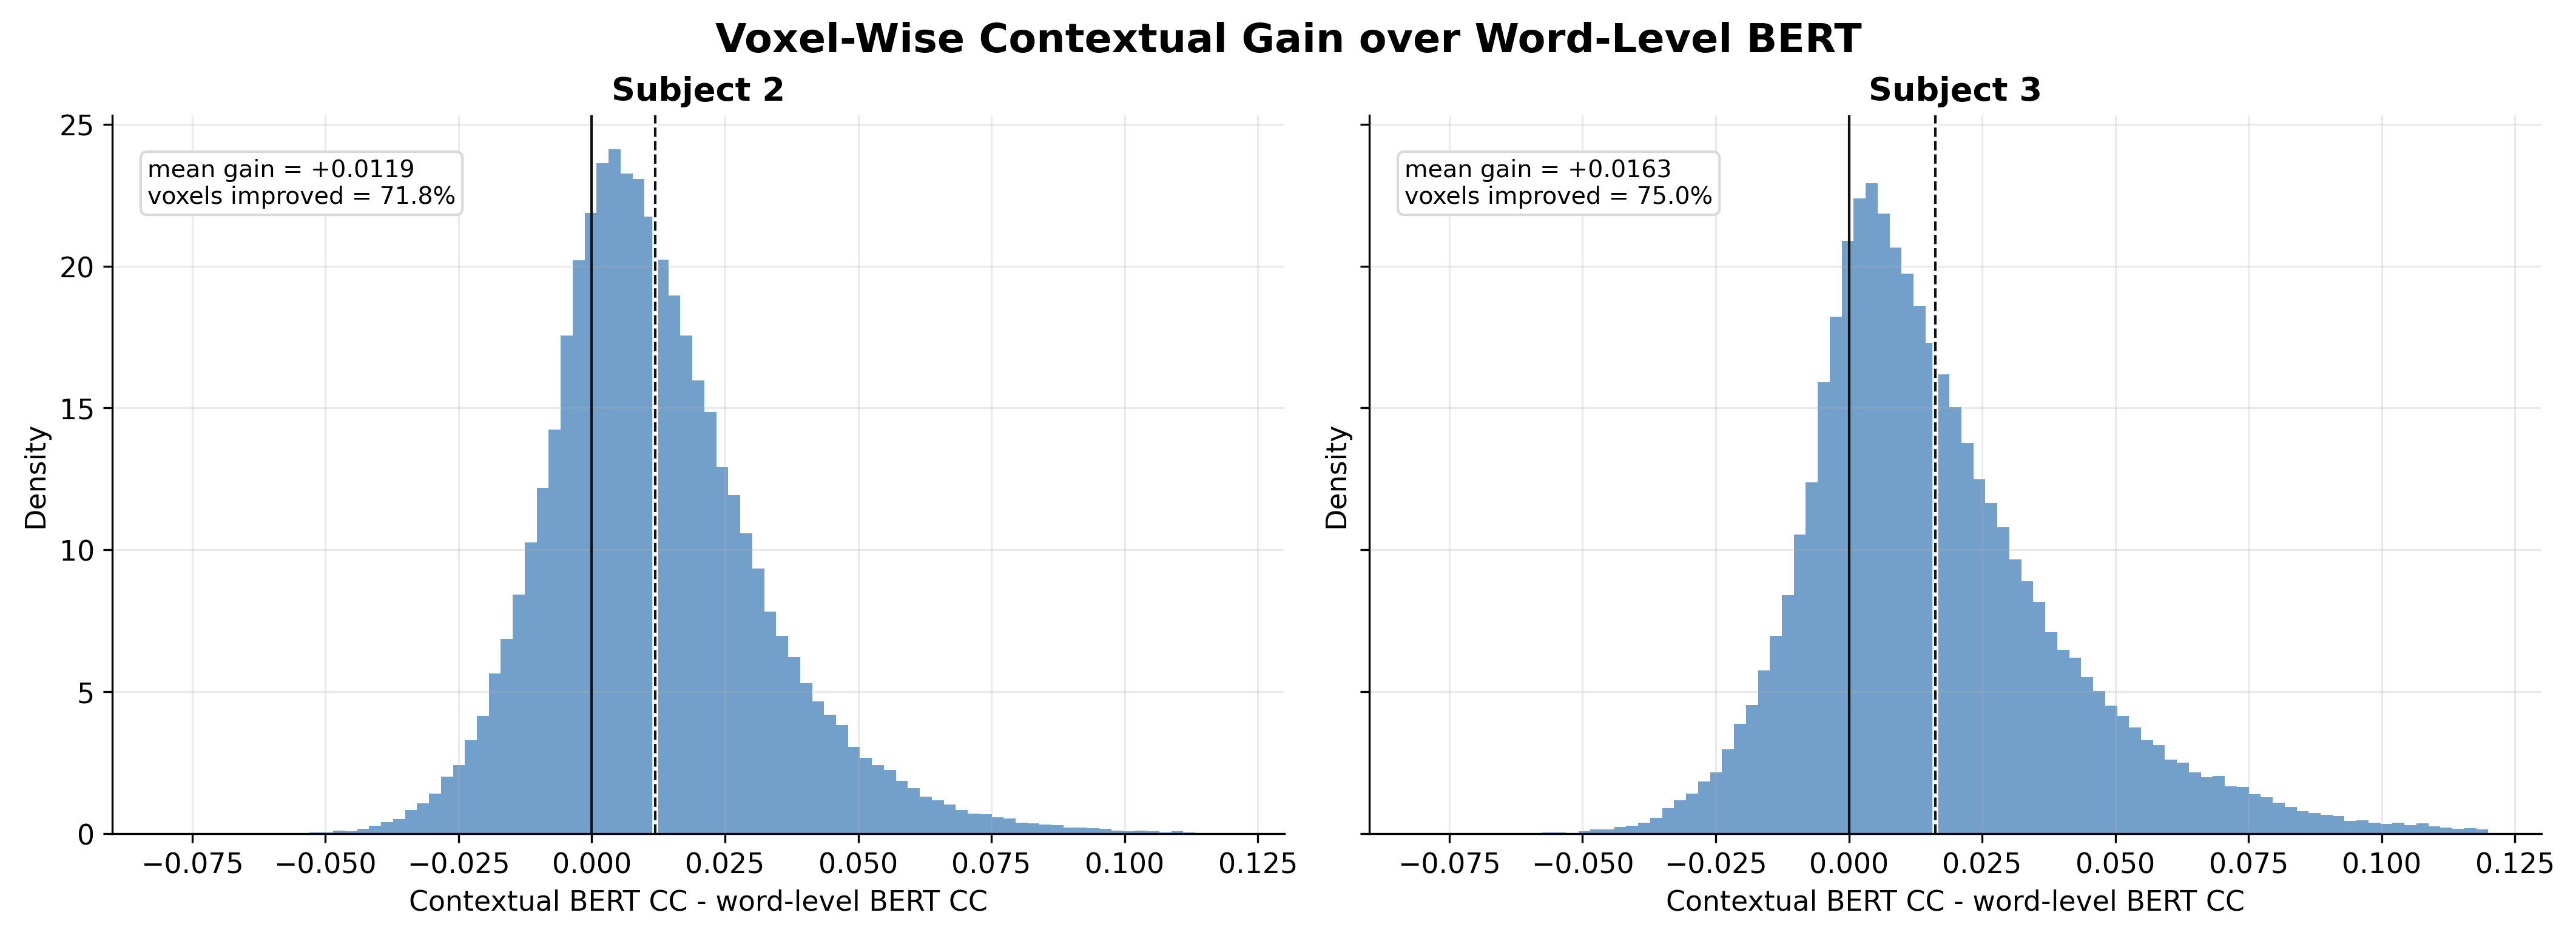
\includegraphics[width=\textwidth]{../figures/lab32/stability_contextual_vs_wordlevel_delta.png}
    \caption{Voxel-wise gain from contextual BERT over word-level BERT. Each histogram shows \(\mathrm{CC}_{\mathrm{contextual}} - \mathrm{CC}_{\mathrm{wordlevel}}\) across voxels. The solid vertical line marks zero gain, and the dashed line marks the mean gain. Contextual BERT improves 71.8\% of voxels for Subject 2 and 75.0\% for Subject 3, showing that the improvement is broad rather than being driven only by a few extreme voxels.}
    \label{fig:context-stability-delta}
\end{figure}

To check whether this improvement was driven by only a small number of voxels, we also examined voxel-wise CC differences between contextual BERT and word-level BERT. Figure~\ref{fig:context-stability-delta} shows the distribution of
\[
\Delta \mathrm{CC}_v =
\mathrm{CC}_{v,\mathrm{contextual}} -
\mathrm{CC}_{v,\mathrm{wordlevel}}.
\]
For Subject 2, the mean voxel-wise gain is \(+0.0119\), and 71.8\% of voxels improve. For Subject 3, the mean gain is \(+0.0163\), and 75.0\% of voxels improve. Thus, contextual BERT does not only improve the aggregate metrics, it shifts most voxel-wise CC values upward.

This stability check shows that the main BERT result depends on preserving story context during embedding extraction. When much less context is provided, prediction accuracy drops substantially for both subjects. This supports our modeling choice that BERT's advantage is not simply that it provides high-dimensional pretrained vectors, but that it can represent words in their surrounding narrative context. In that sense, the contextual BERT result is stable across subjects and metrics, but it is sensitive to removing the linguistic context that BERT is designed to use.

\subsection{LoRA Rank Stability}
\label{sec:stability-lora-rank}
We also tested whether the LoRA fine-tuning results depended strongly on the adapter rank. Our main LoRA model used rank \(r=8\). As a stability check, we trained and evaluated two additional LoRA models with \(r=4\) and \(r=16\), keeping the same training stories, MLM objective, embedding extraction pipeline, and ridge regression procedure. The smaller rank uses fewer trainable parameters, while the larger rank gives the adapter more capacity.

\begin{table}[H]
\centering
\begin{tabular}{llrrrr}
\toprule
Subject & LoRA Rank & Mean CC & Median CC & Top 5\% CC & Top 1\% CC \\
\midrule
Subject 2 & \(r=4\) & 0.0209 & 0.0156 & 0.0728 & 0.1146 \\
Subject 2 & \(r=8\) & 0.0213 & 0.0158 & 0.0732 & 0.1162 \\
Subject 2 & \(r=16\) & 0.0218 & 0.0159 & 0.0764 & 0.1180 \\
\midrule
Subject 3 & \(r=4\) & 0.0336 & 0.0248 & 0.1049 & 0.1574 \\
Subject 3 & \(r=8\) & 0.0327 & 0.0236 & 0.1051 & 0.1610 \\
Subject 3 & \(r=16\) & 0.0319 & 0.0232 & 0.1029 & 0.1593 \\
\bottomrule
\end{tabular}
\caption{LoRA rank stability results. The main model uses \(r=8\); \(r=4\) and \(r=16\) are stability checks.}
\label{tab:lora-rank-stability}
\end{table}

The LoRA rank results were stable across \(r=4\), \(r=8\), and \(r=16\) (Table~\ref{tab:lora-rank-stability}). For Subject 2, performance increased slightly with rank, but the differences were small. Mean CC ranged only from 0.0209 to 0.0218, and top 1\% CC ranged from 0.1146 to 0.1180. For Subject 3, the pattern was not monotonic. Rank \(r=4\) had the highest mean CC, rank \(r=8\) had the highest top 5\% CC and top 1\% CC, and rank \(r=16\) remained very close to both. Using a bigger LoRA rank did not reliably make the model better. Therefore, our original LoRA rank choice was reasonable, and the results do not seem to depend on accidentally choosing one rank.

Figure~\ref{fig:lora-rank-metrics} further shows that the LoRA rank curves are relatively flat. Subject 2 has a slight upward trend as rank increases, while Subject 3 shows a slight decrease in mean and median CC as rank increases. However, these changes are small compared with the overall gap between contextual BERT-style models and the non-contextual baselines in section~\ref{sec:stability-context}. This suggests that the main conclusion about LoRA is stable. LoRA performs similarly to full fine-tuning and pretrained BERT while updating only a small fraction of the BERT parameters.

\begin{figure}[H]
\centering
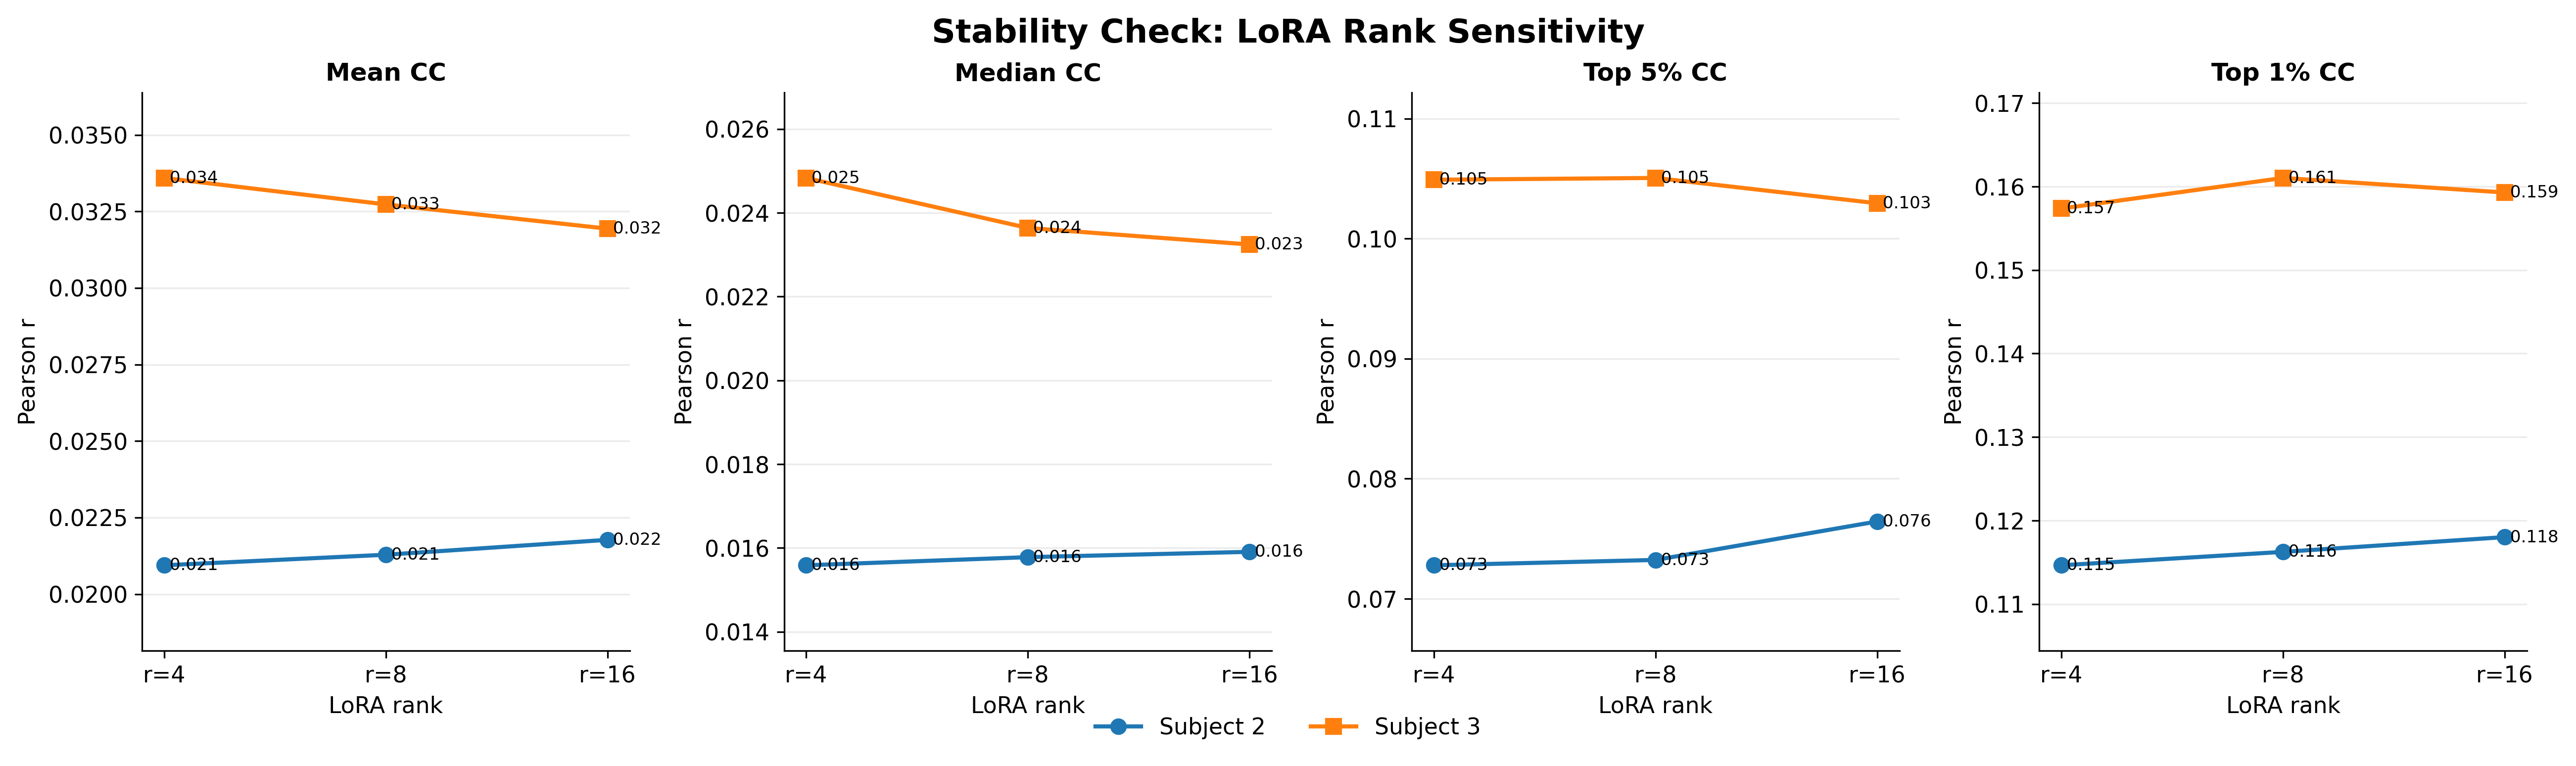
\includegraphics[width=\textwidth]{../figures/lab32/stability_lora_rank_metrics.png}
\caption{LoRA rank sensitivity across summary metrics. Lines show performance for \(r=4\), \(r=8\), and \(r=16\) separately for each subject. The curves are nearly flat, especially compared with the larger differences between embedding families in the main results, indicating that the LoRA conclusions are not highly sensitive to rank.}
\label{fig:lora-rank-metrics}
\end{figure}

Overall, these two stability analyses support the main modeling decisions. The contextual BERT check shows that preserving surrounding language context meaningfully improves prediction over isolated word-level BERT embeddings. The LoRA rank check shows that the parameter-efficient fine-tuning results are stable across reasonable adapter ranks. As a result, our final interpretation focuses on contextual BERT-based models and treats the \(r=8\) LoRA model as a representative parameter-efficient alternative rather than as a finely tuned special case.

\section{Discussion}
The main finding is not simply that BERT performs best, but that the type of linguistic information represented by the embedding matters. BoW captures word identity, GloVe and Word2Vec capture context-independent semantic similarity, and BERT captures how a word is used in context. The consistent ordering across both subjects suggests that fMRI responses during story listening are better predicted by representations that preserve contextual meaning rather than by isolated word identity or static word semantics.

At the same time, the improvement is concentrated rather than brain-wide. Mean and median CCs remain low for every model, while the top-percentile metrics increase much more under BERT. This pattern is important because it suggests that contextual embeddings are not making all voxels slightly better in the same way. Instead, they are most useful for a subset of voxels whose responses are already more tied to the language stimulus. This is consistent with the idea that language encoding is spatially selective, such that many voxels contain little text-predictable signal, while a smaller set carries reliable story-related information.

The fine-tuning results were more subtle. Full fine-tuning and LoRA did not consistently outperform pretrained BERT, even though they were adapted to the training stories. One explanation is that the training corpus was too small relative to the size of BERT, so fine-tuning added little stable information beyond what the pretrained model already encoded. This does not mean fine-tuning is useless in general. Rather, in this setting, the pretrained representation was already strong enough that additional adaptation had inconsistent benefits. LoRA is still useful to discuss because it reached performance close to full fine-tuning while training far fewer parameters. That makes it a parameter-efficient alternative, even though it did not produce a clear predictive gain.

The stability checks sharpen this interpretation. When BERT was given much less surrounding story context during embedding extraction, prediction performance dropped substantially. This suggests that the advantage of BERT is not just that it provides high-dimensional pretrained vectors. The surrounding narrative context itself matters. In contrast, changing the LoRA rank did not produce a consistent improvement, suggesting that our conclusions are not strongly dependent on one LoRA rank choice.

The interpretability results should be read more cautiously than the prediction results. SHAP and LIME identified some words that were clearly related to each story, such as food-system and inequality words in \textit{canplanetearthfeedtenbillionpeople} and medical-event words in \textit{stumblinginthedark}. However, they also highlighted common function words and showed limited agreement overall. This means the explanations are useful for generating hypotheses about what story content matters for high-CC voxels, but they should not be treated as direct evidence that a voxel responds to an isolated word. The most convincing interpretability evidence comes from words that are story-relevant, appear in high-CC voxels, and are supported by more than one explanation method.

\subsection{Limitations}
Several limitations affect how strongly we can interpret these results. First, prediction accuracy is modest in absolute terms, especially when averaged across all voxels. This is expected for noisy whole-brain fMRI data, but it means the strongest claims should focus on the high-CC voxel subset rather than the entire brain. Second, our validation design uses a fixed held-out test-story split for final evaluation, while ridge regularization is selected using bootstrap chunks within the training set. Although this is a reasonable fixed-holdout evaluation strategy, we did not use the full leave-one-story-out cross-validation (LOSO CV), which might provide a more comprehensive assessment of story-to-story variability in model performance. Third, the fine-tuning data are limited. With more stories, more subjects, or more extensive hyperparameter tuning, full fine-tuning and LoRA might show different behavior. Fourth, SHAP and LIME are perturbation-based approximations. Removing or masking words changes the surrounding BERT context, so word importance reflects the effect of perturbing the story input, not a direct neural response to an isolated word. Finally, because the model includes HRF delays, an important word may partly reflect nearby narrative content that influences later BOLD responses.

\section{Conclusion}
This project tested whether different text representations can predict fMRI responses while subjects listened to natural stories. The answer is yes, but only for a subset of voxels and only modestly in absolute terms. BoW carried little predictive signal, GloVe and Word2Vec improved performance, and contextual BERT embeddings performed best across both subjects.

The strongest conclusion is that contextual information matters. BERT improved prediction more than static embeddings, especially among the best-predicted voxels. Fine-tuning and LoRA did not clearly outperform pretrained BERT, suggesting that pretrained contextual representations were already strong for this task. LoRA was still a useful comparison because it achieved performance close to full fine-tuning while training far fewer parameters.

The SHAP and LIME analyses suggest that the best-predicted voxels are sensitive to story-relevant words, but the interpretations should be treated cautiously. Some important words were semantically meaningful and aligned with each story's content, while others were function words or method-specific artifacts. Agreement between SHAP and LIME was limited overall, though some local agreement appeared for specific high-CC voxels in \textit{stumblinginthedark}. Taken together, the results support the main hypothesis that contextual language representations better predict language-evoked brain responses than non-contextual representations, while also showing that reliable interpretation requires focusing on high-CC voxels and stable word-level patterns.

\appendix
\section{Appendix}
\subsection{Additional Figures}
\begin{figure}[H]
    \centering
    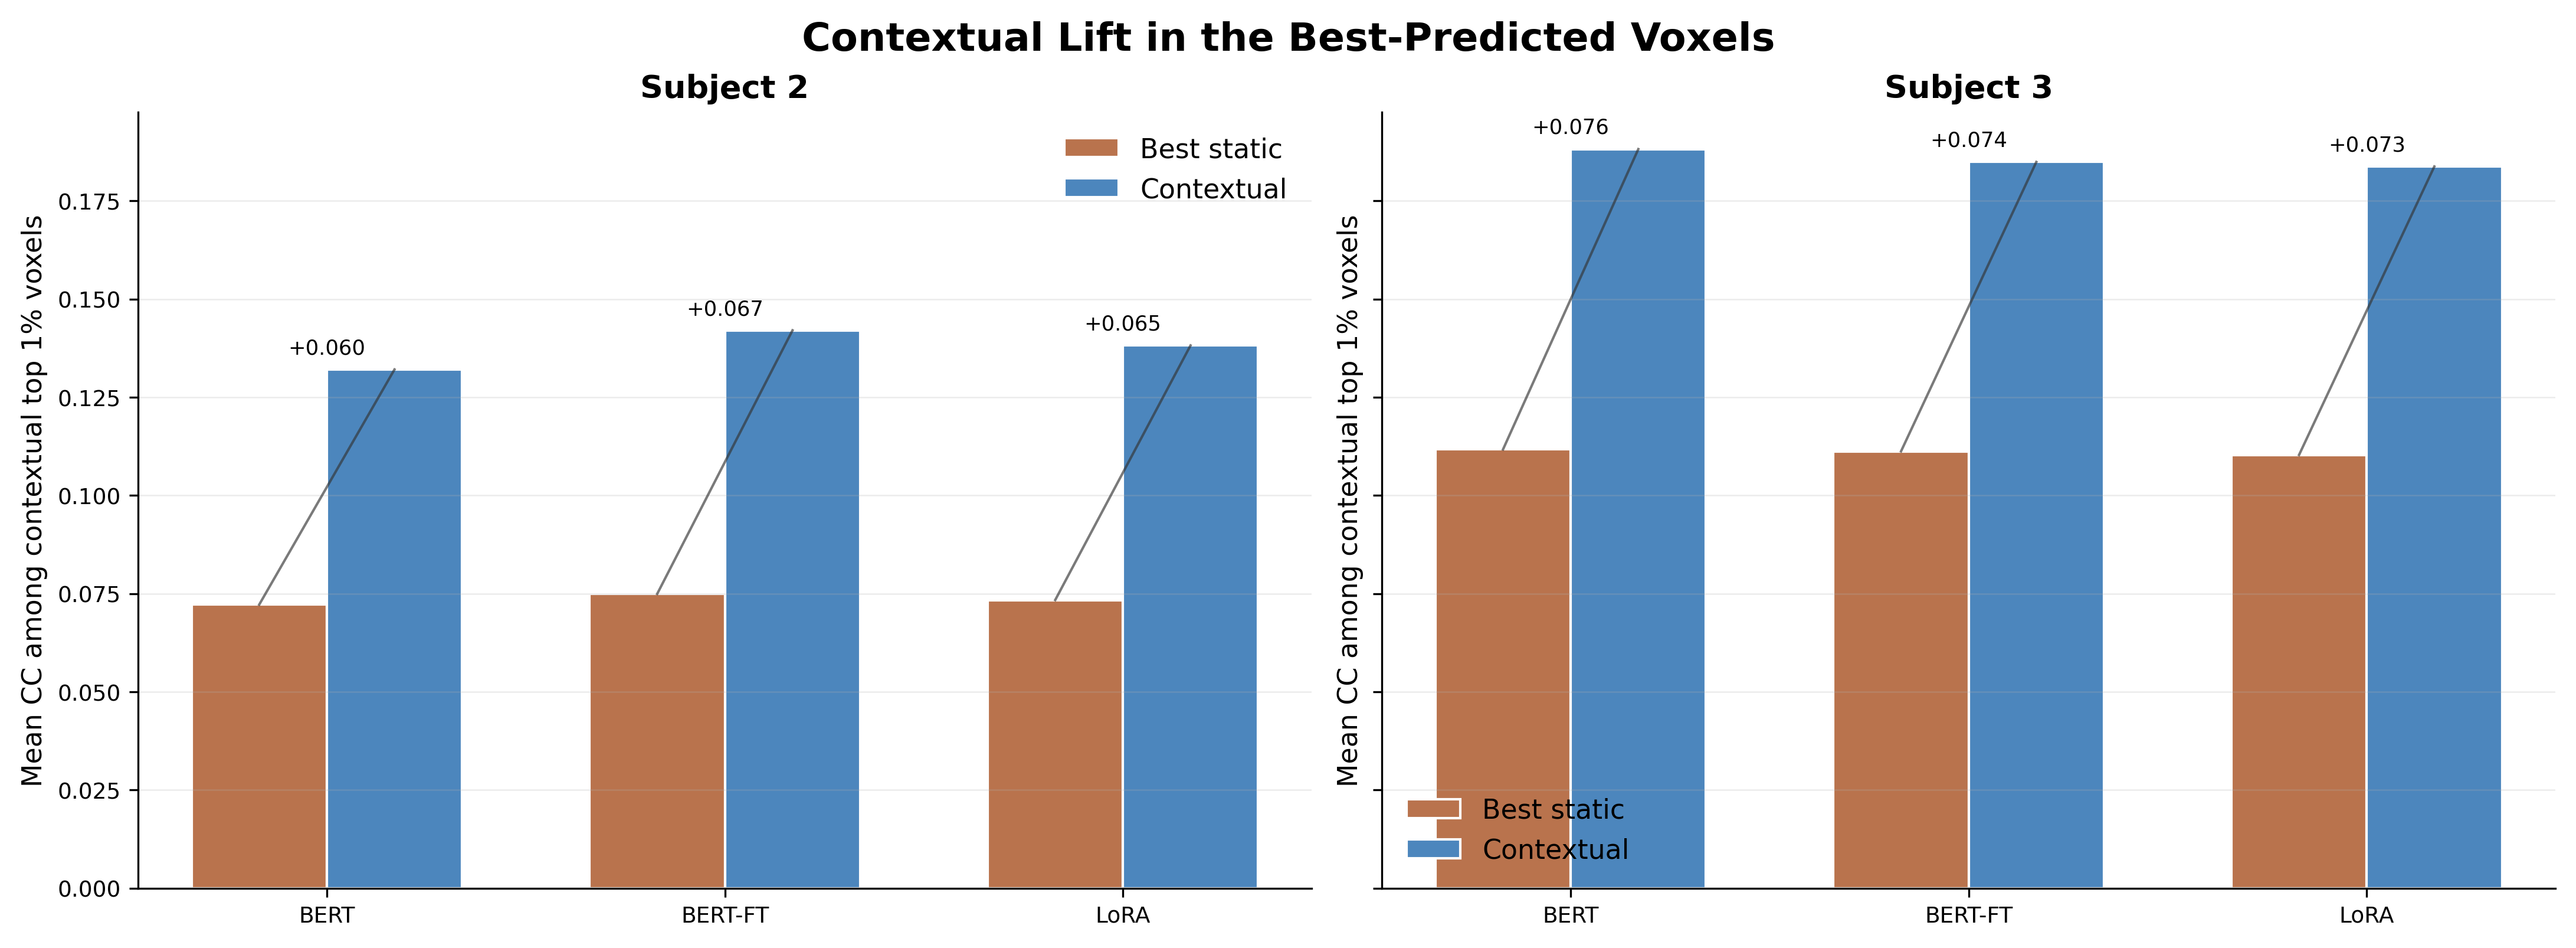
\includegraphics[width=\textwidth]{../figures/lab32/fig6_top_voxel_contextual_lift.png}
    \caption{For each contextual BERT variant, we compare its mean CC on its top 1\% of predicted voxels (blue) against the best static embedding on the same voxels (orange); the annotated gap is the contextual lift. The lift is consistent across BERT, BERT-FT, and LoRA for both subjects, confirming that the contextual advantage is not an artifact of a favorable voxel subset.}
    \label{fig:contextual_lift_appendix}
    \end{figure}

\begin{figure}[H]
    \centering
    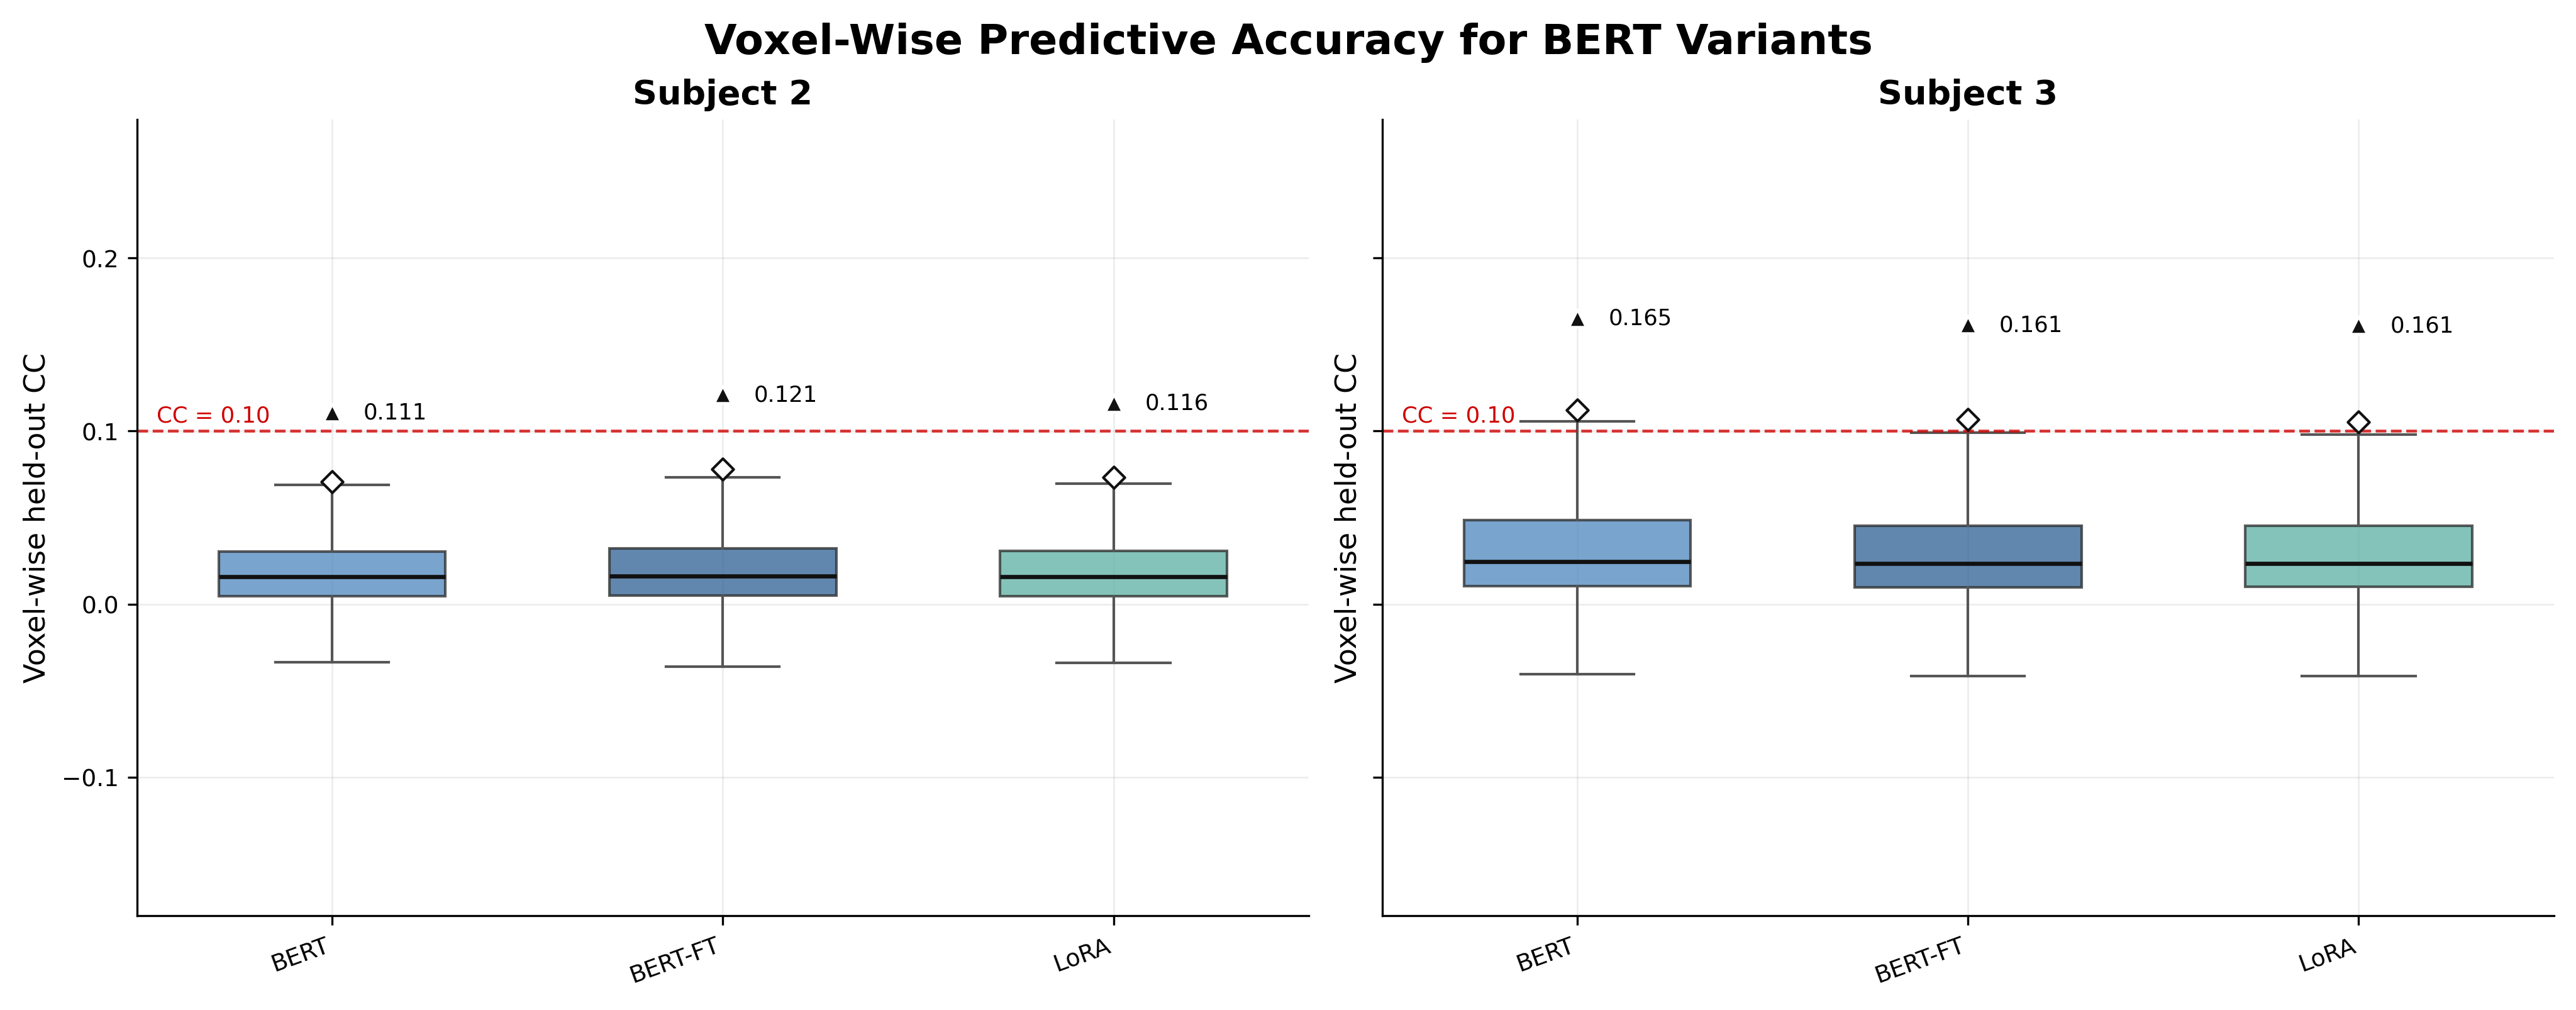
\includegraphics[width=\textwidth]{../figures/lab32/fig2_bert_voxel_distributions.png}
    \caption{Voxel-wise held-out CC distributions for the three BERT variants. The red dashed line marks the CC \(=0.10\) interpretation threshold. For both subjects, all three BERT variants have top 1\% CC values above this threshold, while the medians remain far below it. This shows that reliable prediction is concentrated in a small upper-tail subset of voxels, motivating our focus on high-CC voxels for SHAP and LIME.}
    \label{fig:bert_distributions_appendix}
    \end{figure}

\begin{figure}[H]
    \centering
    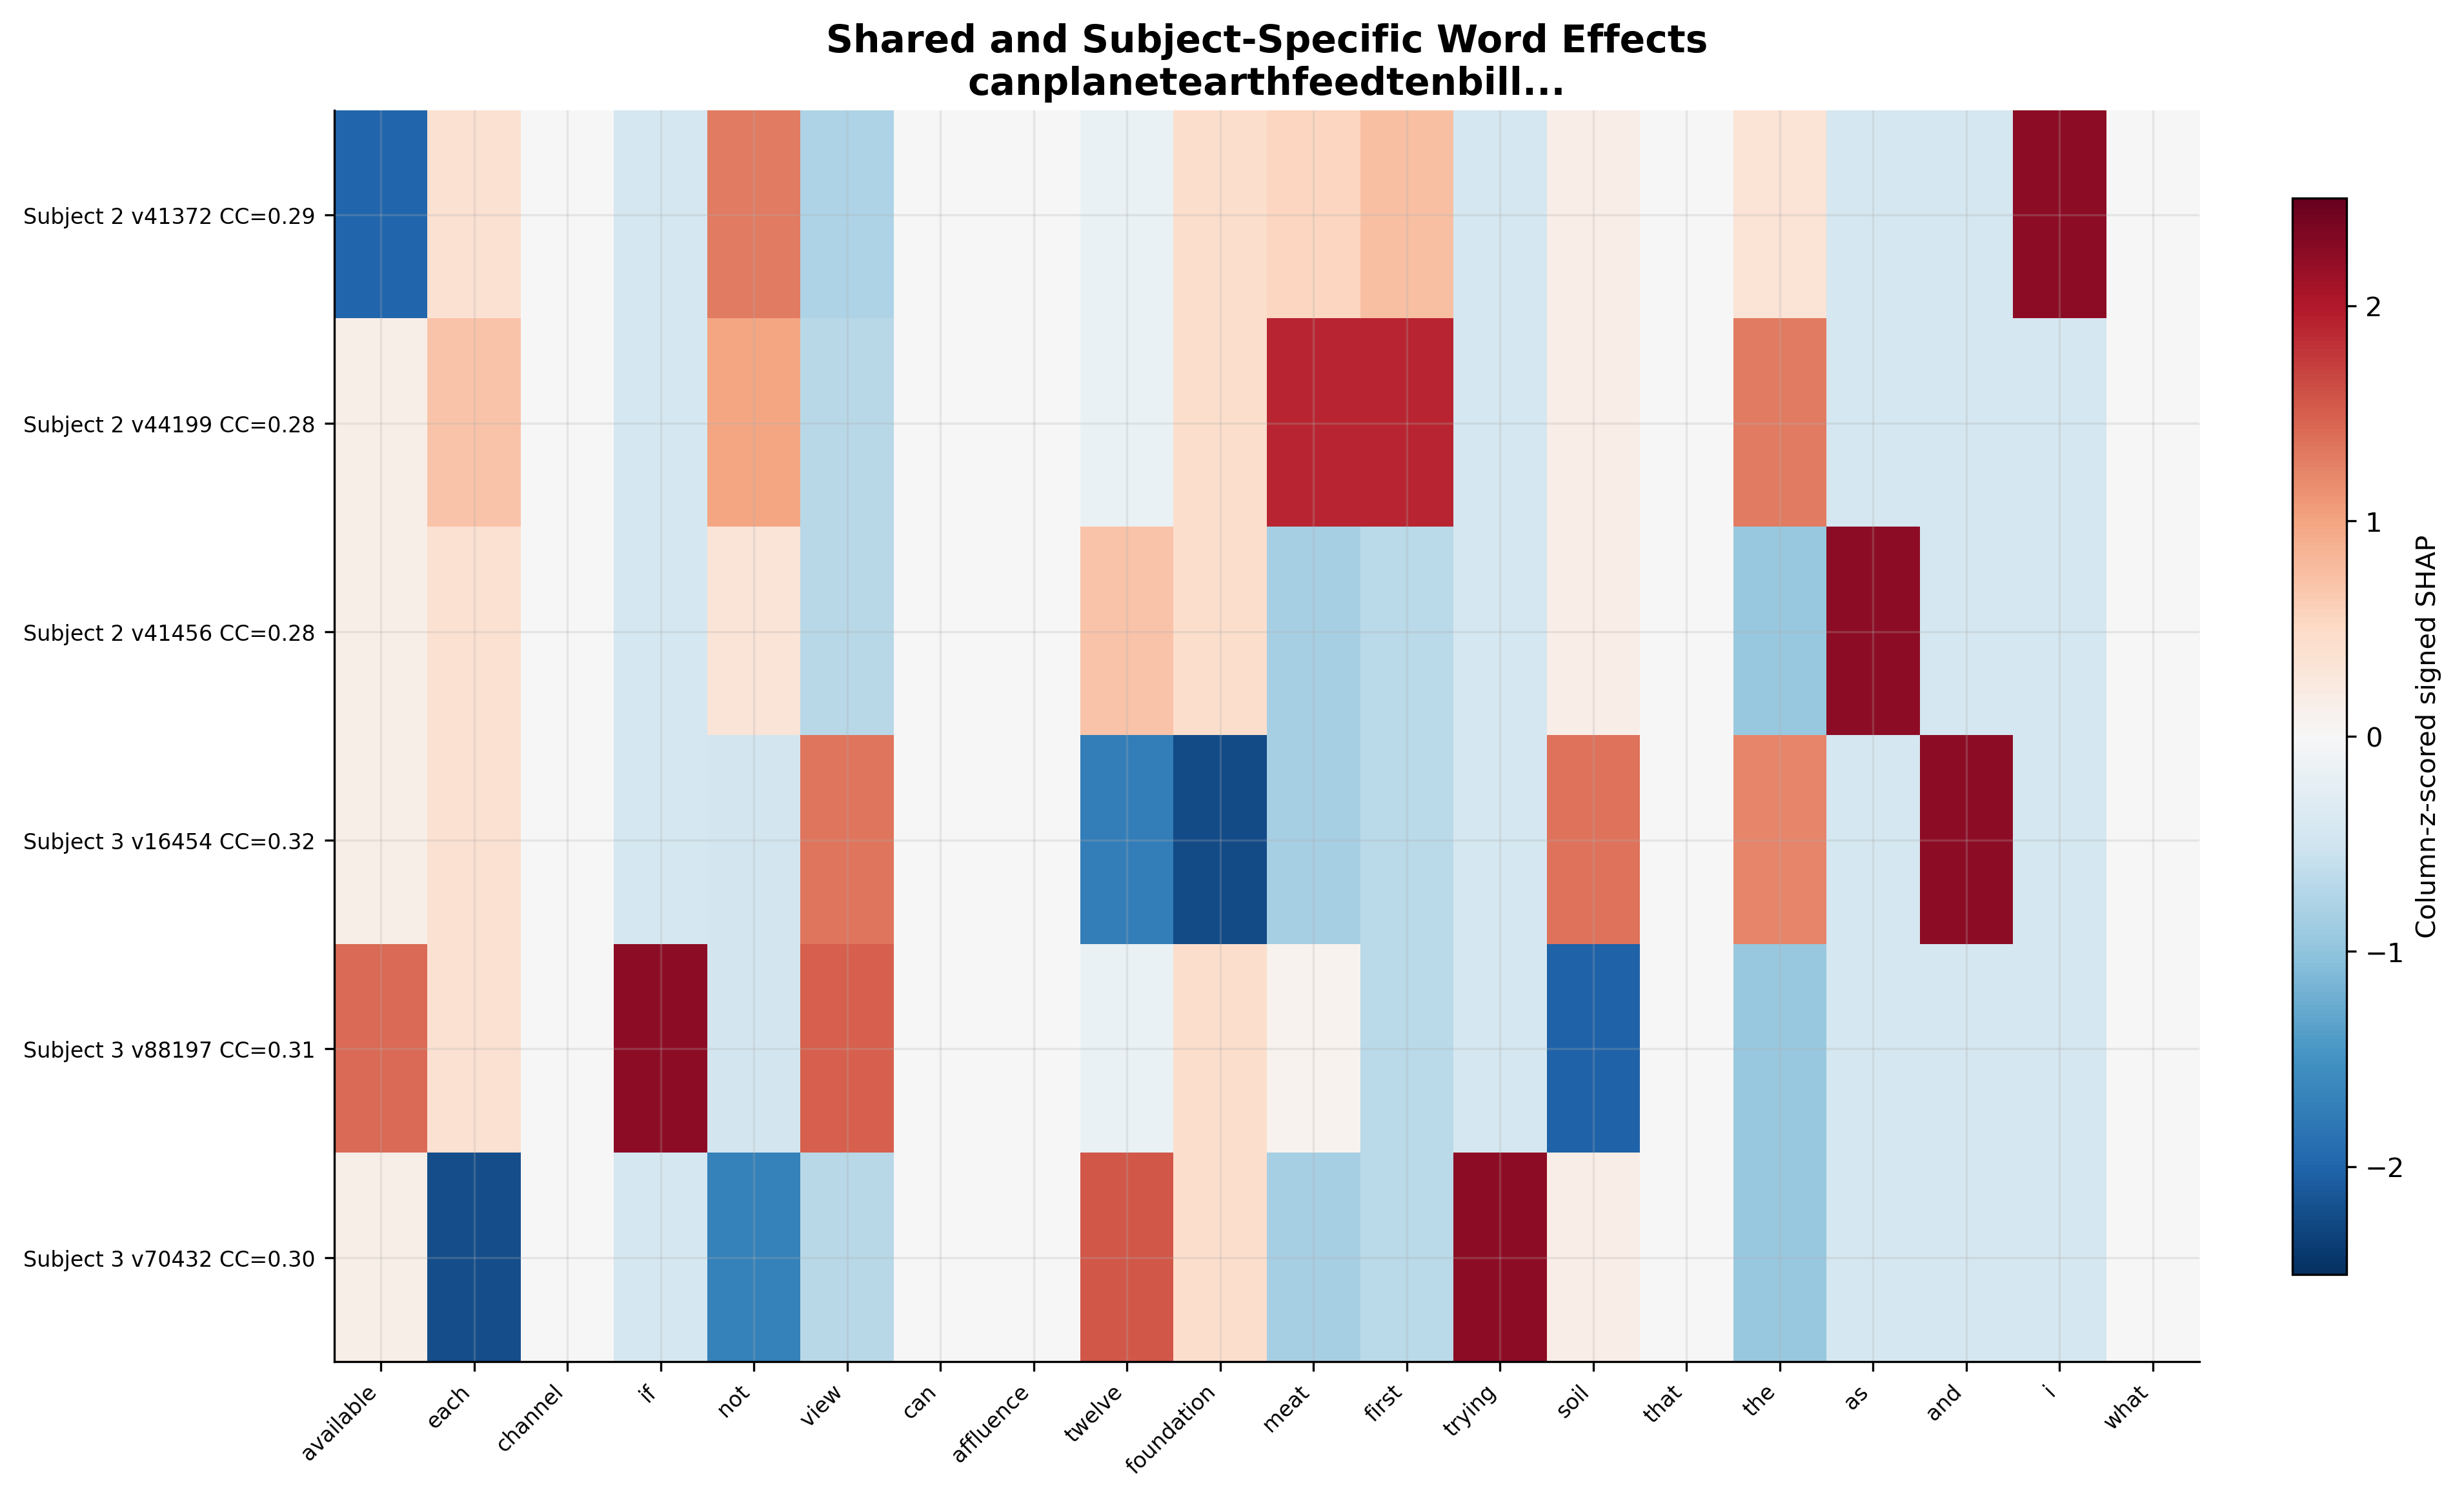
\includegraphics[width=0.85\textwidth]{../figures/lab33/fig4_heatmap_story1.png}
    \caption{Heatmap of column-z-scored signed SHAP values for \textit{canplanetearthfeedtenbillionpeople}. Rows are selected high-CC voxels, and columns are top-ranked words pooled across voxels. Red indicates relatively positive signed SHAP values and blue indicates relatively negative signed SHAP values, compared within each word. The patchy pattern shows that word effects are mostly voxel-specific rather than shared across all selected voxels.}
    \label{fig:heatmap_story1_appendix}
\end{figure}

\begin{figure}[H]
    \centering
    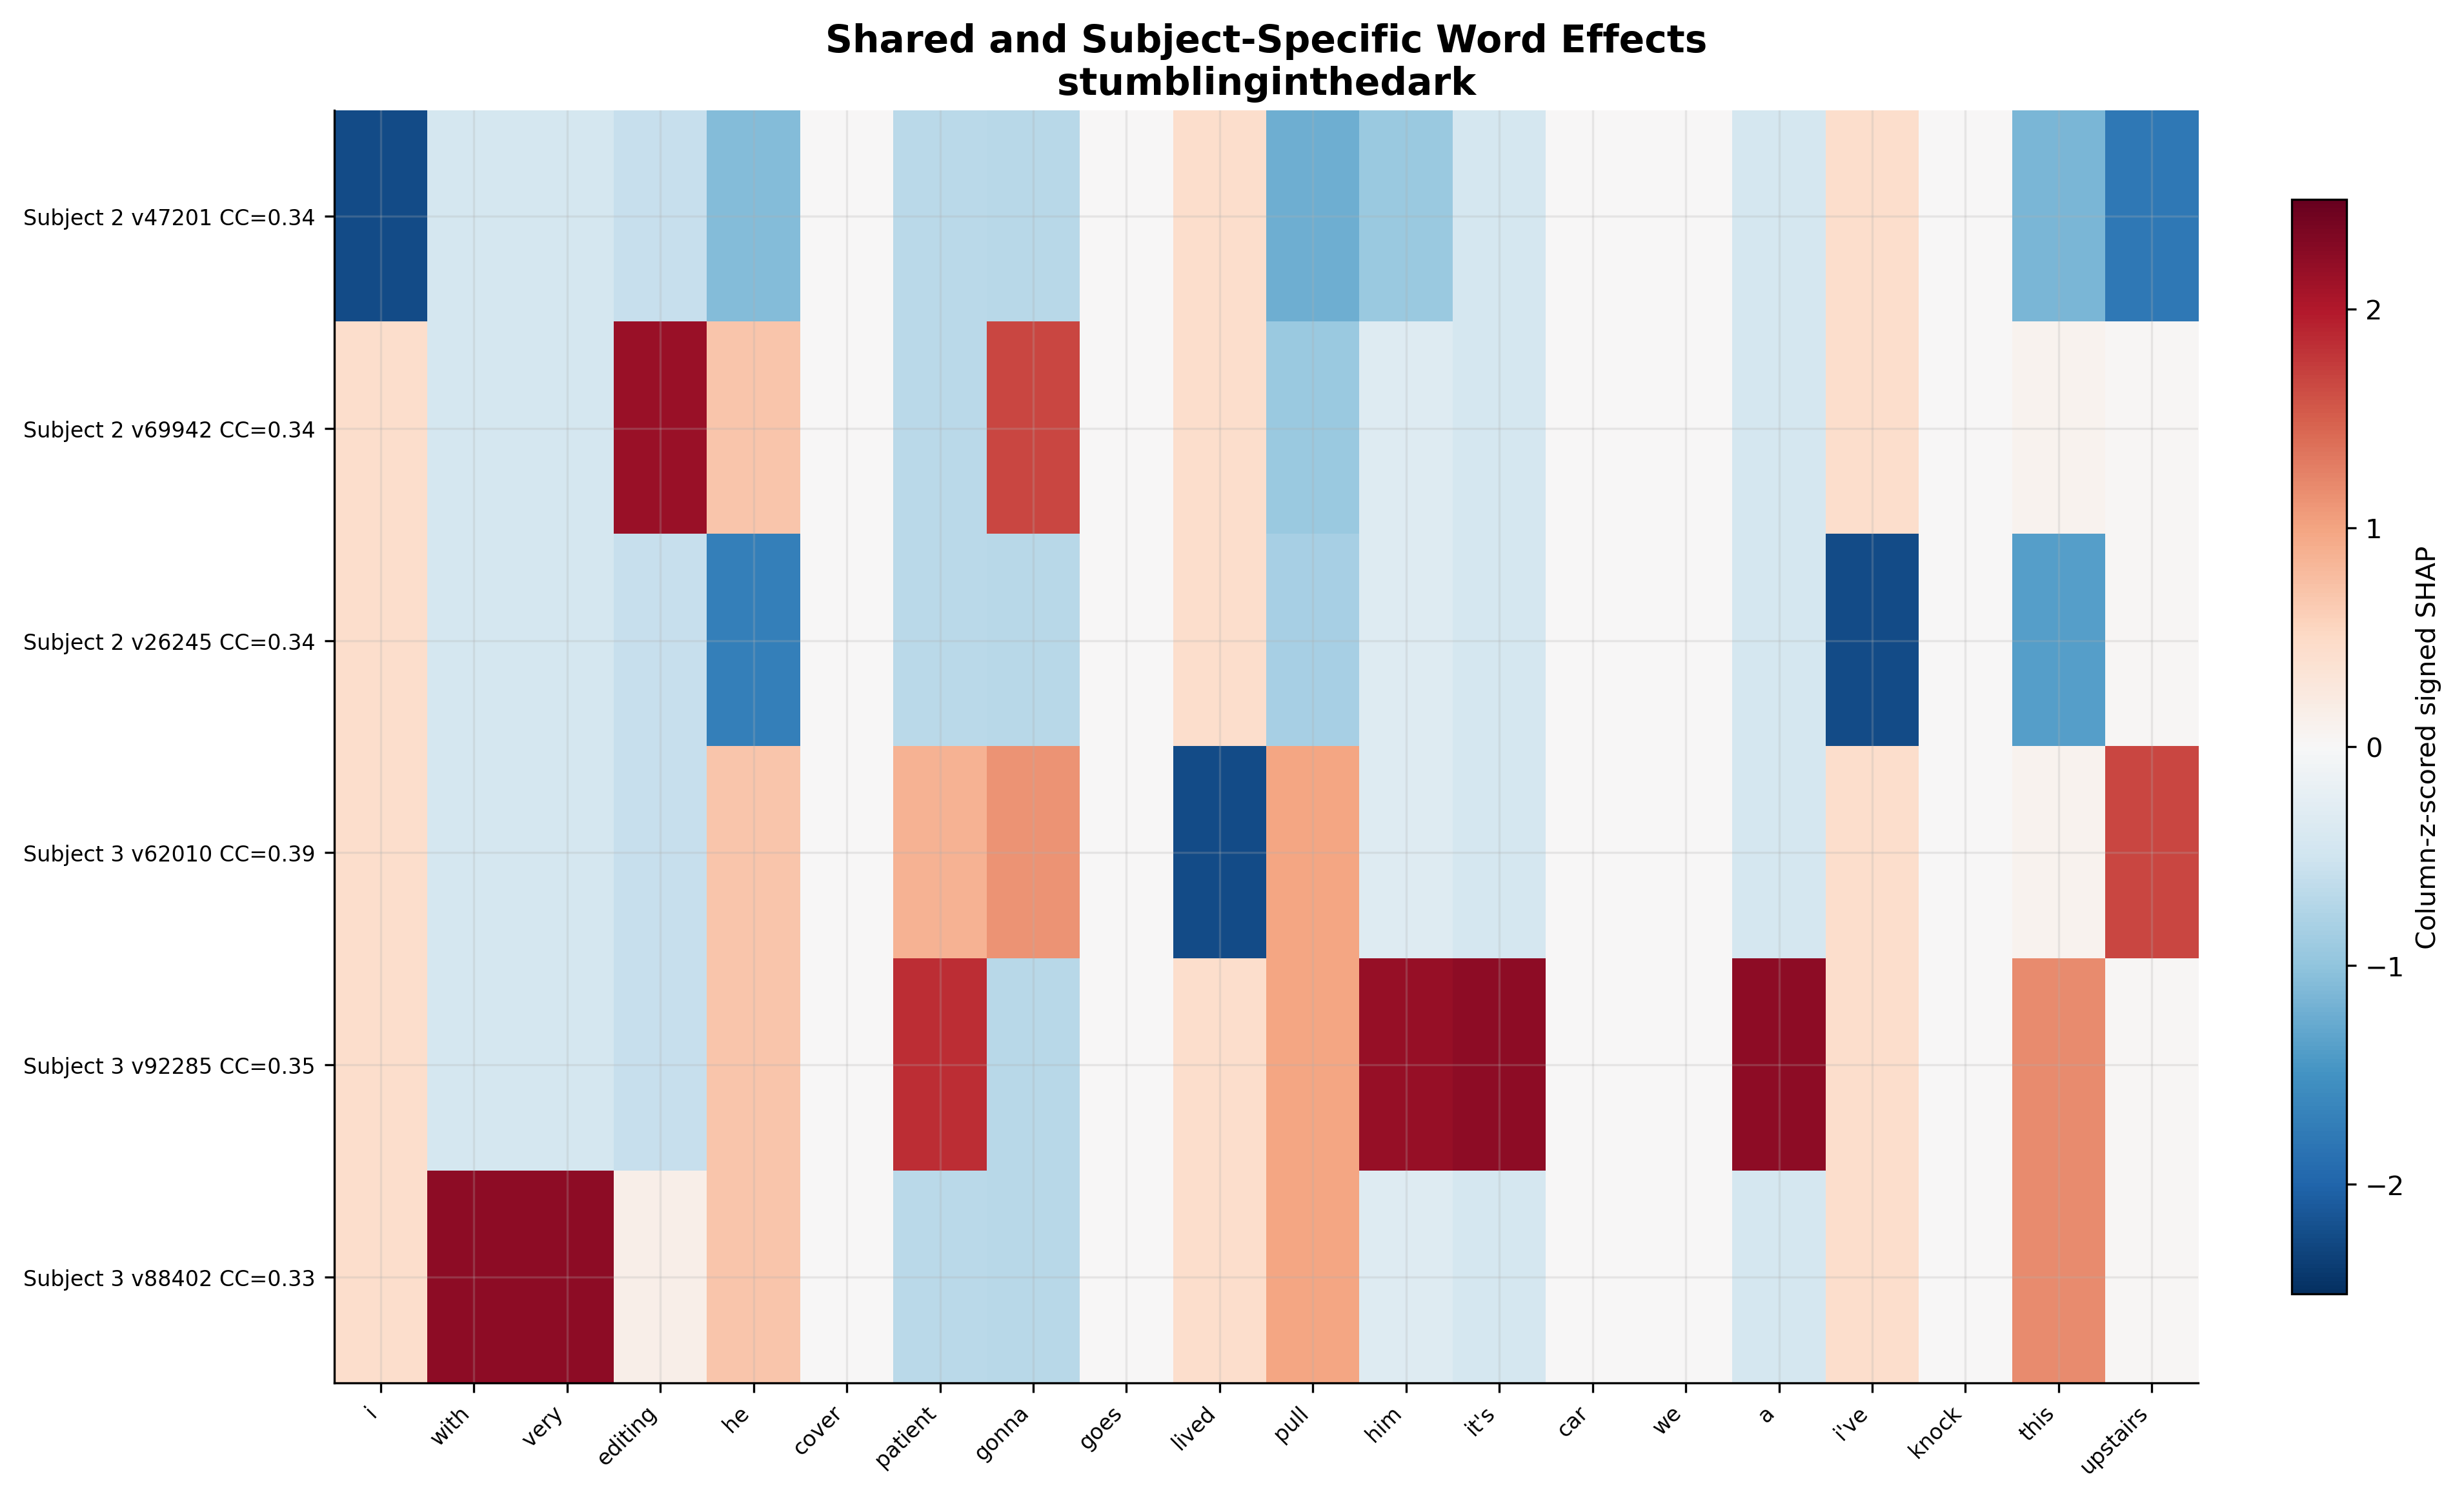
\includegraphics[width=0.85\textwidth]{../figures/lab33/fig4_heatmap_story2.png}
    \caption{Heatmap of column-z-scored signed SHAP values for \textit{stumblinginthedark}. Rows are selected high-CC voxels, and columns are top-ranked words. Event-related words such as \textit{knock}, \textit{refrigerator}, \textit{car}, \textit{ambulance}, and \textit{affected} appear in the selected word set, but their signed SHAP values vary across voxels and subjects. This supports the interpretation that the explanations are partly story-relevant but remain voxel-specific.}
    \label{fig:heatmap_story2_appendix}
\end{figure}

\section{Bibliography}
\bibliographystyle{plainnat}
\begin{thebibliography}{9}

\bibitem[Jain and Huth(2018)]{jain2018}
S.\ Jain and A.\ G.\ Huth.
Incorporating context into language encoding models for fMRI.
\emph{bioRxiv}, 2018.
\url{https://doi.org/10.1101/327601}

\bibitem[Hu et al.(2022)]{hu2022lora}
E.\ J.\ Hu, Y.\ Shen, P.\ Wallis, Z.\ Allen-Zhu, Y.\ Li, S.\ Wang, L.\ Wang,
and W.\ Chen.
LoRA: Low-rank adaptation of large language models.
\emph{ICLR}, 2022.

\bibitem{yu2024}
Yu, B. and Barter, R. L. (2024).
\textit{Veridical Data Science: The Practice of Responsible Data Analysis and Decision Making}.
MIT Press.

\end{thebibliography}

\section{Academic honesty}
\subsection{Statement}
We affirm that the work presented in this report is our own and that all sources used, including discussions with classmates and use of computational tools, are properly cited. Academic research honesty is necessary because scientific progress depends on the integrity of reported results. When researchers misrepresent their methods or findings, it undermines the ability of others to build on that work, wastes resources, and erodes public trust in science. Addressed to Professor Bin Yu.

\subsection{LLM Usage}
\subsubsection*{Coding}
Claude, Codex, and GitHub Copilot were used to assist with code documentation, inline commenting, debugging, and script organization. All analytical decisions, algorithmic choices, and implementation logic were our own. We reviewed and verified the correctness of all suggested code before including it in the final project.

\subsubsection*{Writing}
Claude, ChatGPT, and Grammarly were used to assist with grammar revisions, clarity, and general editing. All ideas, interpretations, and written content are our own. All AI-assisted revisions were reviewed and approved by us before submission.
\end{document}